\documentclass[titlepage, a4paper]{article}
\usepackage[swedish]{babel}
\usepackage[utf8]{inputenc}
\usepackage{color}
\usepackage{graphicx}
\usepackage{etoolbox}
\usepackage{stringenc}
\usepackage{pdfescape}

% Sidformat
\usepackage{a4wide}

% Fixa Appendix-titlar
\usepackage[titletoc,title]{appendix}

% Bättre tabeller
\usepackage{tabularx}

% Bättre bildtexter
\usepackage[margin=10pt,font=small,labelfont=bf,labelsep=endash]{caption}

% Enkelt kommando som låter mig attgöra-markera text
\newcommand{\todo}[1] {\textbf{\textcolor{red}{#1}}}

% Nytt \paragraph låter oss ha onumrerade bitar
\makeatletter
\renewcommand\paragraph{\@startsection{paragraph}{4}{\z@}%
{-3.25ex\@plus -1ex \@minus -.2ex}%
{1.5ex \@plus .2ex}%
{\normalfont\normalsize\bfseries}}
\makeatother

%\providecommand{\LIPSlogga}{../mall/logga1.png}
\providecommand{\LIPSdatum}{\today}

%% Headers och Footers
\usepackage{fancyhdr}
\pagestyle{fancy}
%\lhead{\includegraphics[scale=0.4]{\LIPSlogga}}
\rhead{\ifdef{\LIPSutfardare}{Utfärdat av \LIPSutfardare \\\LIPSdatum}\LIPSdatum}
\lfoot{\LIPSkursnamn \\ \LIPSdokumenttyp}
\cfoot{\thepage}
\rfoot{\LIPSprojektgrupp \\ \LIPSprojektnamn}

%% Titelsida
\newcommand{\LIPSTitelsida}{%
{\ }\vspace{45mm}
\begin{center}
  \textbf{\Huge \LIPSdokument}
\end{center}
\begin{center}
  {\Large Redaktör: \LIPSredaktor}
\end{center}
\begin{center}
  {\Large \textbf{Version \LIPSversion}}
\end{center}
\vfill
\begin{center}
  {\large Status}\\[1.5ex]
  \begin{tabular}{|*{3}{p{40mm}|}}
    \hline
    Granskad & \LIPSgranskare & \LIPSgranskatdatum \\
    \hline
    Godkänd & \LIPSgodkannare & \LIPSgodkantdatum \\
    \hline
  \end{tabular}
\end{center}
\newpage
}

% Projektidentitet
\newenvironment{LIPSprojektidentitet}{%
{\ }\vspace{45mm}
\begin{center}
  {\Large PROJEKTIDENTITET}\\[0.5ex]
  {\small
  \LIPSartaltermin, \LIPSprojektgrupp\\
  Linköpings Tekniska Högskola, IDA
  }
\end{center}
\begin{center}
  {\normalsize Gruppdeltagare}\\
  \begin{tabular}{|l|l|p{25mm}|l|}
    \hline
    \textbf{Namn} & \textbf{Ansvar} & \textbf{Telefon} & \textbf{E-post} \\
    \hline
}%
{%
    \hline
  \end{tabular}
\end{center}
\begin{center}
  {\small
    \ifdef{\LIPSgruppadress}{\textbf{E-postlista för hela gruppen}: \LIPSgruppadress\\}{}
    \ifdef{\LIPSgrupphemsida}{\textbf{Hemsida}: \LIPSgrupphemsida\\[1ex]}{}
    \ifdef{\LIPSkund}{\textbf{Kund}: \LIPSkund\\}{}
    \ifdef{\LIPSkundkontakt}{\textbf{Kontaktperson hos kund}: \LIPSkundkontakt\\}{}
    \ifdef{\LIPSkursansvarig}{\textbf{Kursansvarig}: \LIPSkursansvarig\\}{}
    \ifdef{\LIPShandledare}{\textbf{Handledare}: \LIPShandledare\\}{}
  }
\end{center}
\newpage
}
\newcommand{\LIPSgruppmedlem}[4]{\hline {#1} & {#2} & {#3} & {#4} \\}

%% Dokumenthistorik
\newenvironment{LIPSdokumenthistorik}{%
\begin{center}
  Dokumenthistorik\\[1ex]
  %\begin{small}
    \begin{tabular}{|l|l|p{60mm}|l|l|}
      \hline
      \textbf{Version} & \textbf{Datum} & \textbf{Utförda förändringar} & \textbf{Utförda av} & \textbf{Granskad} \\
      }%
    {%
			\hline
    \end{tabular}
  %\end{small}
\end{center}
}

\newcommand{\LIPSversionsinfo}[5]{\hline {#1} & {#2} & {#3} & {#4} & {#5} \\}

% Kravlistor
\newenvironment{LIPSkravlista}{
	\center
		\tabularx{\textwidth}{| p{1.2cm} | p{1.9cm} | X | c |}
			\hline
			\textbf{Krav} & \textbf{Förändring} & \textbf{Beskrivning} & \textbf{Prioritet} \\\hline
}
{
		\endtabularx
	\endcenter
}

\newcounter{LIPSkravnummer}
\addtocounter{LIPSkravnummer}{1}
\newcommand{\LIPSkrav}[4][Krav \arabic{LIPSkravnummer}]{{#1} & {#2} & {#3} & {#4} \stepcounter{LIPSkravnummer}\\\hline}


% Leveranskravlistor
\newenvironment{LIPSleveranskravlista}{
	\center
		\tabularx{\textwidth}{| p{1.2cm} | p{1.9cm} | X | X |}
			\hline
			\textbf{Krav} & \textbf{Förändring} & \textbf{Beskrivning} & \textbf{Deadline}\\\hline
}
{
		\endtabularx
	\endcenter
}

\newcounter{LIPSleveranskravnummer}
\addtocounter{LIPSleveranskravnummer}{1}
\newcommand{\LIPSleveranskrav}[4][Krav \arabic{LIPSkravnummer}]{{#1} & {#2} & {#3} & {#4} \stepcounter{LIPSkravnummer}\\\hline}


% Milstolps-lista
\newenvironment{LIPSmilstolpar}{
	\center
		\tabularx{\textwidth}{| p{1.2cm} | X | l |}
			\hline
			\textbf{Nr} & \textbf{Beskrivning} & \textbf{Datum} \\\hline
}
{
		\endtabularx
	\endcenter
}

\newcounter{LIPSstolpnummer}
\addtocounter{LIPSstolpnummer}{1}
%\newcommand{\LIPSmilstolpe}[3][Krav \arabic{LIPSstolpnummer}]{{#1} & {#2} & {#3} \stepcounter{LIPSstolpnummer}\\\hline}
\newcommand{\LIPSmilstolpe}[3]{{#1} & {#2} & {#3} \\\hline}

% Aktivitets-lista
\newenvironment{LIPSaktivitetslista}{
	\center
		\tabularx{\textwidth}{| p{0.3cm} | X | c | c | c |}
			\hline
			\textbf{Nr} & \textbf{Beskrivning} & \textbf{Beroende av} & \textbf{Timmar} & \textbf{datum} \\\hline
}
{
		\endtabularx
	\endcenter
}

\newcounter{LIPSaktivitetsnummer}
\addtocounter{LIPSaktivitetsnummer}{1}
% \newcommand{\LIPSaktivitet}[4][\arabic{LIPSstolpnummer}]{{#1} & {#2} & {#3} & {#4} \stepcounter{LIPSstolpnummer}\\\hline}
\newcommand{\LIPSaktivitet}[5]{{#1} & {#2} & {#3} & {#4} & {#5}\\\hline}

% Mall för mötesprotokoll
\newenvironment{projektmote}[2]{
  {\ }\vspace{5mm}

  \centerline{\textbf{\Huge #1}}
  \vspace{2mm}
  \centerline{\LARGE #2}
  \vspace{10mm}

  \begin{itemize}
}
{
  \end{itemize}
}

\newcounter{paragrafnummer}
\addtocounter{paragrafnummer}{1}
\newcommand{\paragraf}[1]{\item{\textsection \arabic{paragrafnummer}. {#1}}\addtocounter{paragrafnummer}{1}}

% Mall för Statusrapport
\newenvironment{statusrapport}{
  \center
    \tabularx{\textwidth}{| p{0.4cm} | X | X | p{14.5mm} | p{13.5mm} | p{16.5mm} | p{16.5mm} |}
    \hline
    \textbf{Nr} & \textbf{Aktivitet} & \textbf{Beroenden} & \textbf{Planerad tid} & \textbf{Nedlagd tid} & \textbf{Planerad klar} & \textbf{Beräknat klart} \\\hline
}
{
    \endtabularx
  \endcenter
}

\newcommand{\aktivitetstatus}[7]{{#1} & {#2} & {#3} & {#4} & {#5} & {#6} & {#7} \\\hline}	% Importera generella layout-strukturer

% Information nödvändig för generella layout-strukturer
\newcommand{\LIPSredaktor}{Johannes Klasson}
\newcommand{\LIPSversion}{P1B}
\newcommand{\LIPSdokument}{Transistor-Level Design Report}
\newcommand{\LIPSdokumenttyp}{Transistor-Level Design Report}
\newcommand{\LIPSgranskatdatum}{2016-03-3}
\newcommand{\LIPSgranskare}{Johannes Klasson}
\newcommand{\LIPSgodkannare}{Martin Nielsen-Lönn}
\newcommand{\LIPSgodkantdatum}{-}
\newcommand{\LIPSkursnamn}{TSEK06}
\newcommand{\LIPSprojektnamn}{16-bit Kogge-Stone Adder}
\newcommand{\LIPSprojektgrupp}{Group 5}
\newcommand{\LIPSartaltermin}{VT, 2016}
\newcommand{\LIPSkund}{ISY}
\newcommand{\LIPSkundkontakt}{Martin Nielsen-Lönn}
\newcommand{\LIPSkursansvarig}{Atila Alvandpour}
\newcommand{\LIPShandledare}{Martin Nielsen-Lönn}

% Dokument-specifika paket
\usepackage{tabularx}
\usepackage{pdfpages}
\usepackage{tikz}
\usepackage{float}
\usetikzlibrary{shapes, arrows}
\usepackage{booktabs} % Horizontal rules in tables
\usepackage[justification=centering]{caption}
\usepackage{adjustbox}
\pagenumbering{roman}


\DeclareGraphicsRule{.0.pdf}{pdf}{*}{}

\begin{document}
\pagenumbering{gobble}
\LIPSTitelsida
\pagenumbering{gobble}
\begin{LIPSprojektidentitet}
  \LIPSgruppmedlem{Johan Isaksson}{Project Leader}{070-2688785}{johis024@student.liu.se}
  \LIPSgruppmedlem{Johannes Klasson}{Document Manager}{073-8209003}{johkl226@student.liu.se}
  \LIPSgruppmedlem{Jonas Tarassu}{VLSI Designer}{070-5738583}{jonta760@student.liu.se}
  \LIPSgruppmedlem{Alexander Yngve}{VLSI Designer}{076-2749762}{aleyn573@student.liu.se}	
\end{LIPSprojektidentitet}

\newpage
\pagenumbering{gobble}
\tableofcontents	%Innehållsförteckning
%\listoffigures
%\listoftables

\newpage
\pagenumbering{gobble}
\begin{LIPSdokumenthistorik}
\LIPSversionsinfo{P1A}{2016-02-19}{First draft}{Johan Isaksson}
\end{LIPSdokumenthistorik}

\newpage
\pagenumbering{arabic}	%Påbörja sidnumrering

% Inledning, översikt osv

\section{Introduction}
This document describes the state of the 16-bit Kogge-Stone adder project in the course TSEK06 after finishing the high level design phase. The system itself is supposed to receive two numbers that should be added together. The result should then both sent out from the system and be compared with a checksum in a BIST (Built-In Self-Test). The meaning of high level is that every basic logic gate is implemented in Verilog-A. The main reason for doing this is to be able to simulate all logic to make sure that everything works as intended. Block level diagrams can be found in section \ref{sec:block_level}, simulation results in section \ref{sec:simulation_results} and a risk analysis in section \ref{sec:risks}. In appendix \ref{app:time_plan} and \ref{app:time_report} a time plan of the next phase and a time report of this phase can be found.


\section{Block Level Description} \label{sec:block_level}
Much of the block level descriptions can be seen in the high level report, but the transistor view of the leaf-cells will be described in this chapter. To find good sizes for our gates we used a very simple sizing strategy. Start small, and if the signal is to weak to drive the components, we just size it up and if necessary, make a buffer for it. The transistor schematic of the basic blocks like AND, OR, DFF etc. are simple enough that we will not include any description for them. \\

In Fig. \ref{top} an updated block diagram of the complete system can be seen.

\begin{figure}[H]
\centering
\captionsetup{justification=centering}
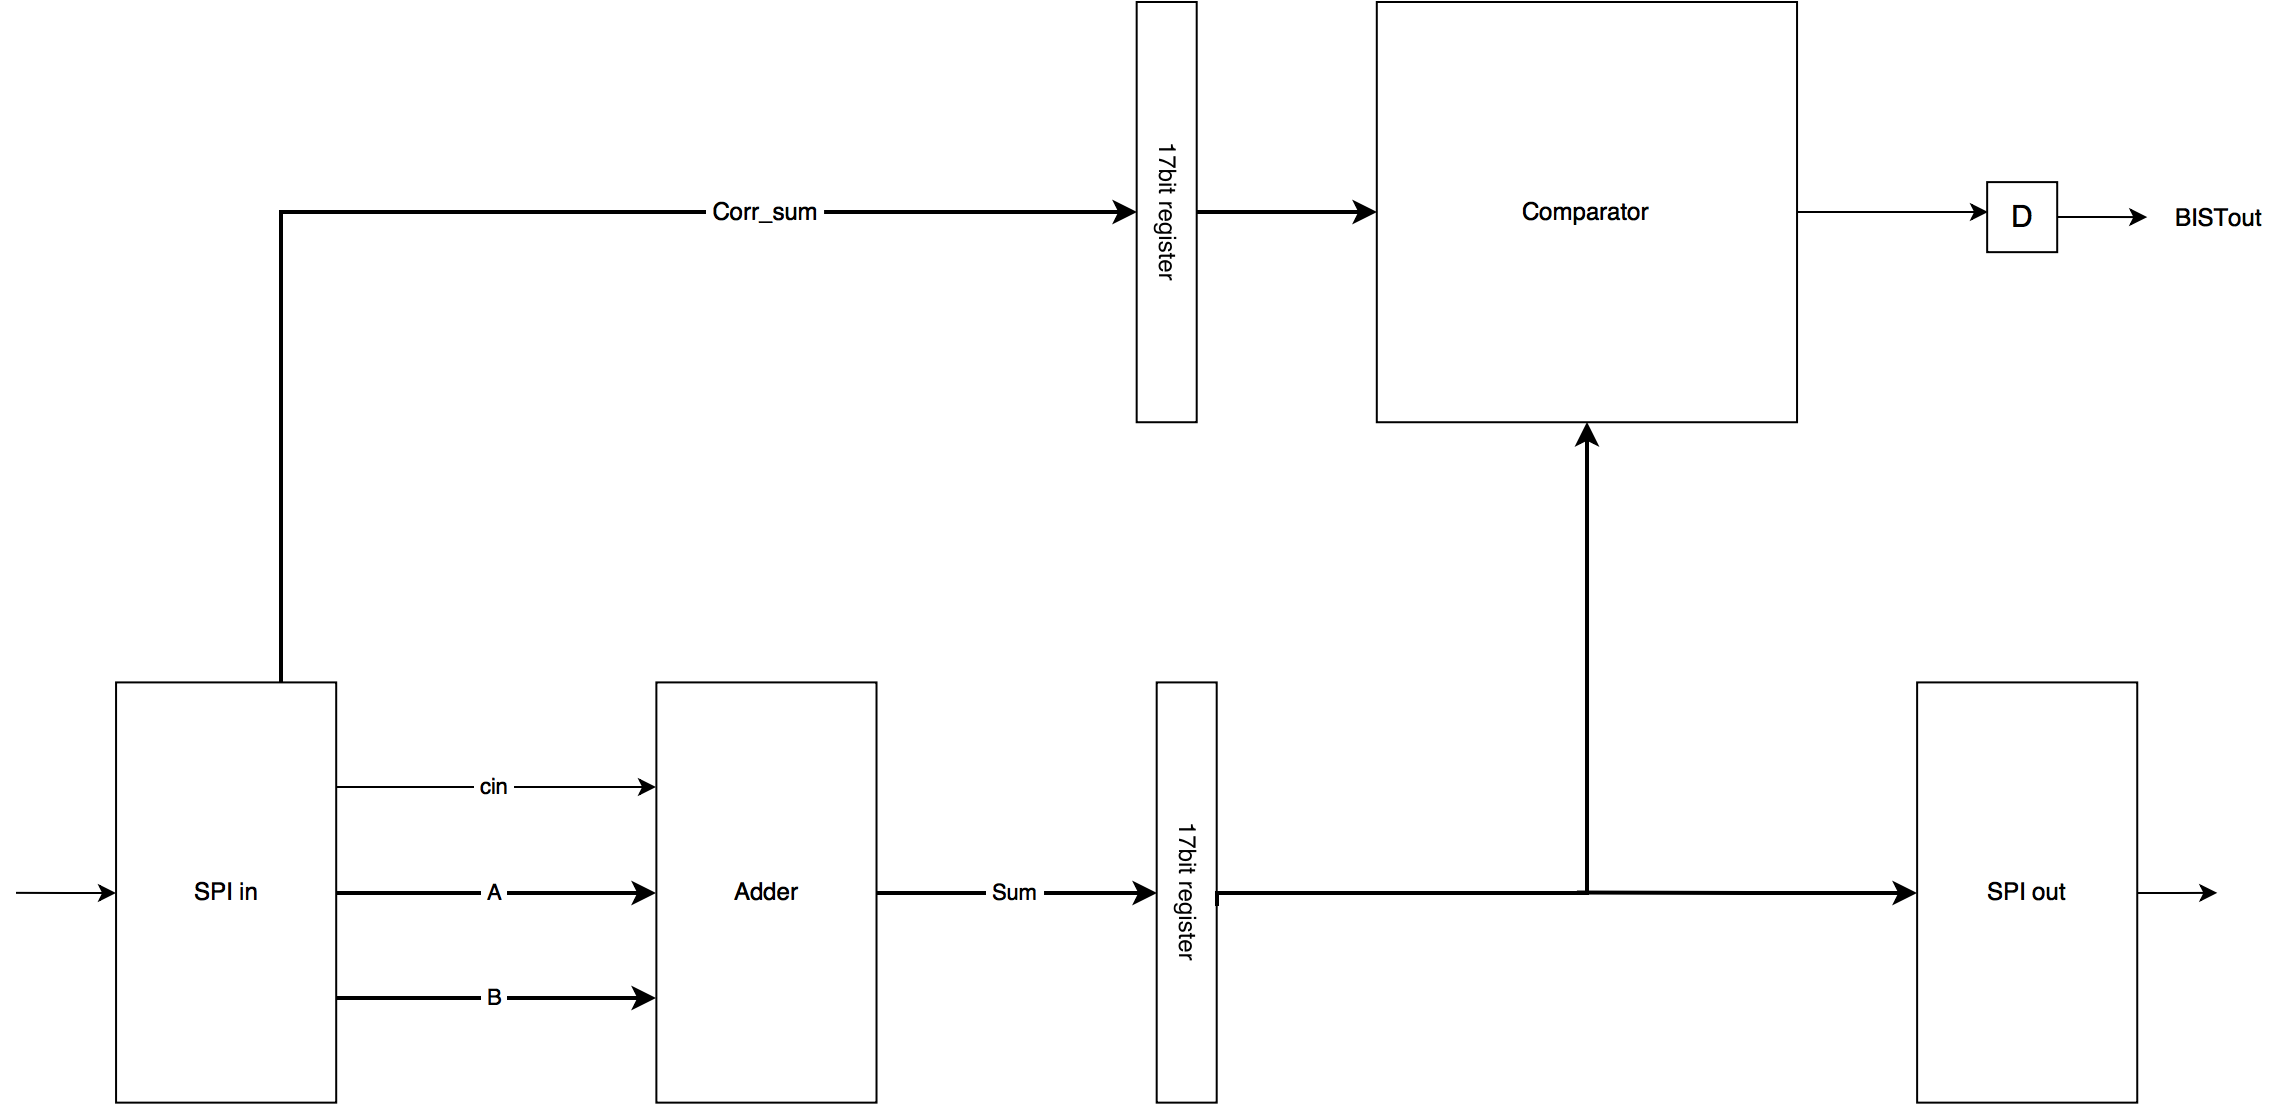
\includegraphics[scale=0.35]{../figures/top_level.png}
\caption{Top level block diagram.}
\label{top}
\end{figure}

The updated diagram contains additional registers for synchronizing the signal before and after the comparator. This was done to provide more stable signals to the comparator and to have a more easily interpreted BISTout signal. The drawback is that the BISTout signal is available two clock cycles after the addition took place.   


\subsection{SPI-in/PRBS}
This module only use basic leaf-cells at the transistor level, so this will be a quite small chapter. There are a few things worth noting regarding the sizing of these basic blocks. Some of the signals are connected to a large amount of devices (60+), which meant that the signal got really weak. This was solved by either just making the gates a bit bigger, or by using a buffer. SPI\_en is using a 9x buffer, SPI\_clk is using a 27x buffer and test\_mode is using a 9x buffer. Clk\_en is the result from an OR gate, and the NOR gate inside it is 6x bigger and the inverter is 18 times bigger. With these modifications, the rise time of the signal was on a healthy level.

\subsection{16-bit Kogge-Stone Adder}
The Kogge-Stone adder consists of four simple blocks connected in a complex way, as can be seen in \ref{app:ks_block}. These four blocks can be seen in figure \ref{fig:red}-\ref{fig:sum}. The red block constitute the initial stage which takes two binary numbers $A$ and $B$ as input. The corresponding truth table is found in table \ref{tab:red} in appendix \ref{app:ks_truth}. The output signals $P$ and $G$ generated from this block are later used by other blocks in the adder. The $G$, also called the Generate signal, trickles down through the hierarchy of yellow, and yellow carry blocks to finally end up in the sum block. The truth table for this block can be found in table \ref{tab:sum}. Truth tables for the yellow and yellow carry blocks are found in table \ref{tab:yellow} and \ref{tab:yellowcarry}.

\begin{figure}[H]
  \centering
  \captionsetup{justification=centering}
  \adjustbox{trim={.3\width} {0\height} {.3\width} {0\height},clip}
  {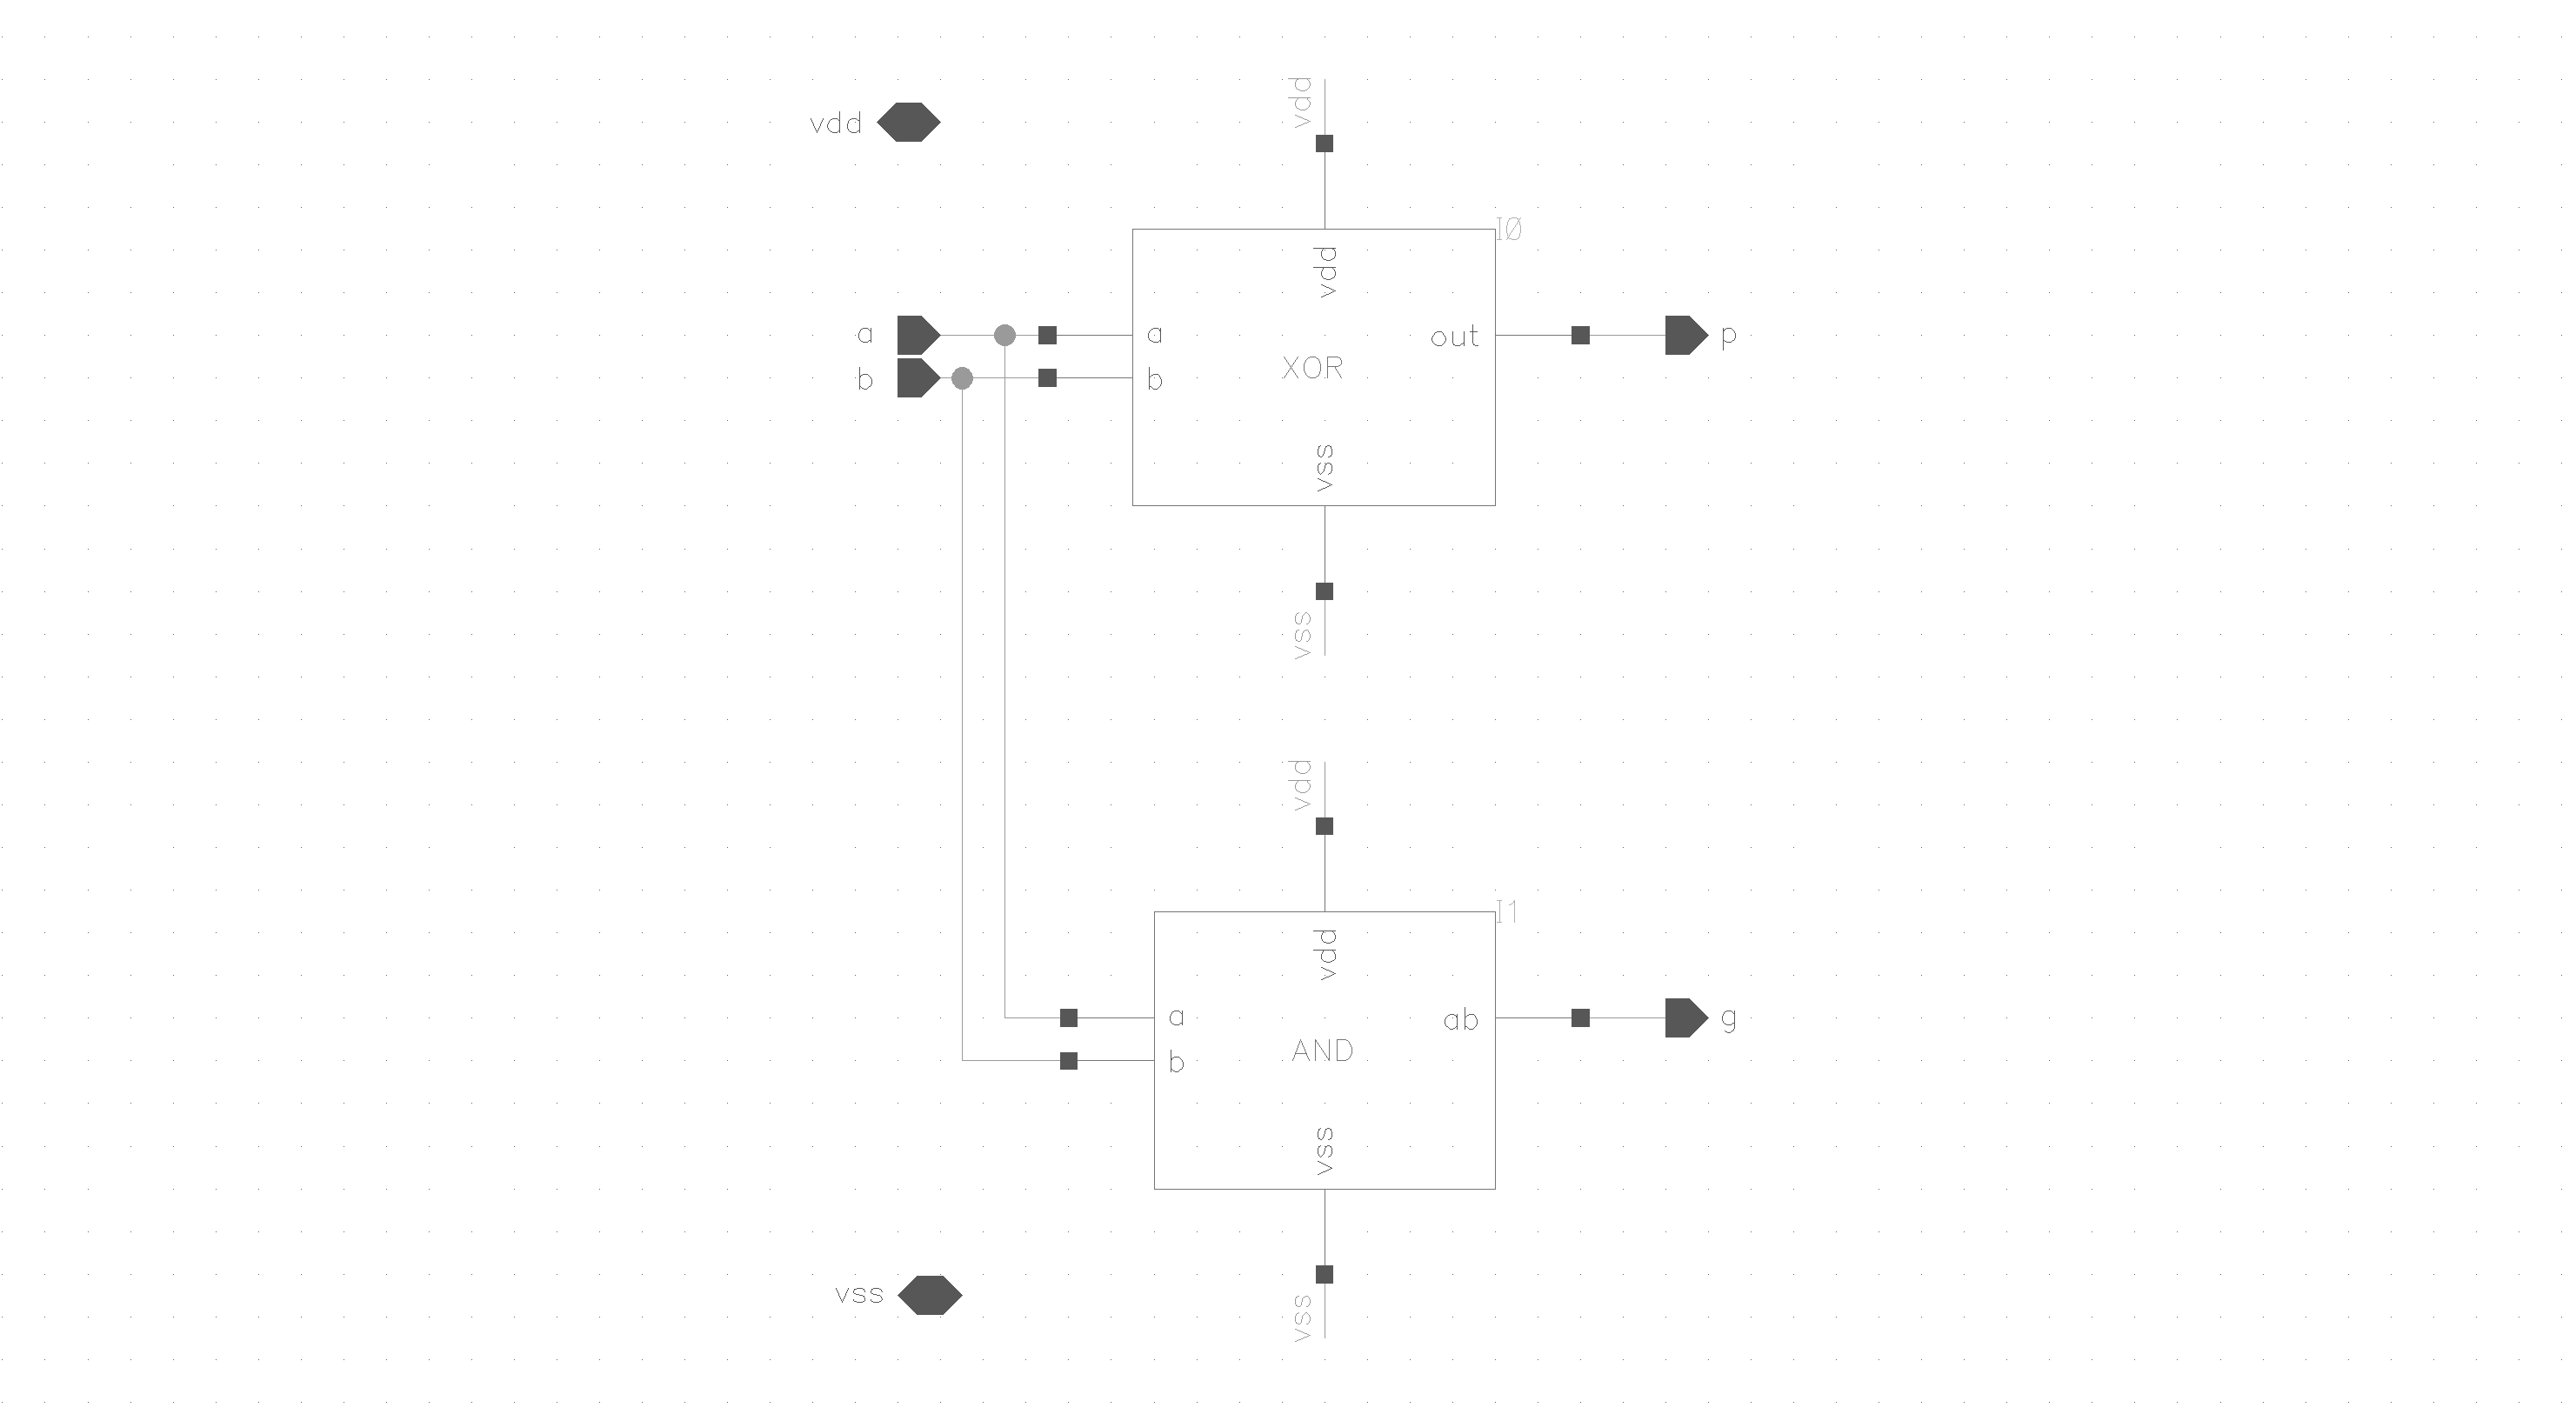
\includegraphics[width=2.0\textwidth]{../figures/red}}
  \caption{Schematic view of the red block.} \label{fig:red}
\end{figure}

\begin{figure}[H]
  \centering
  \captionsetup{justification=centering}
  \adjustbox{trim={.15\width} {0\height} {.12\width} {0\height},clip}
  {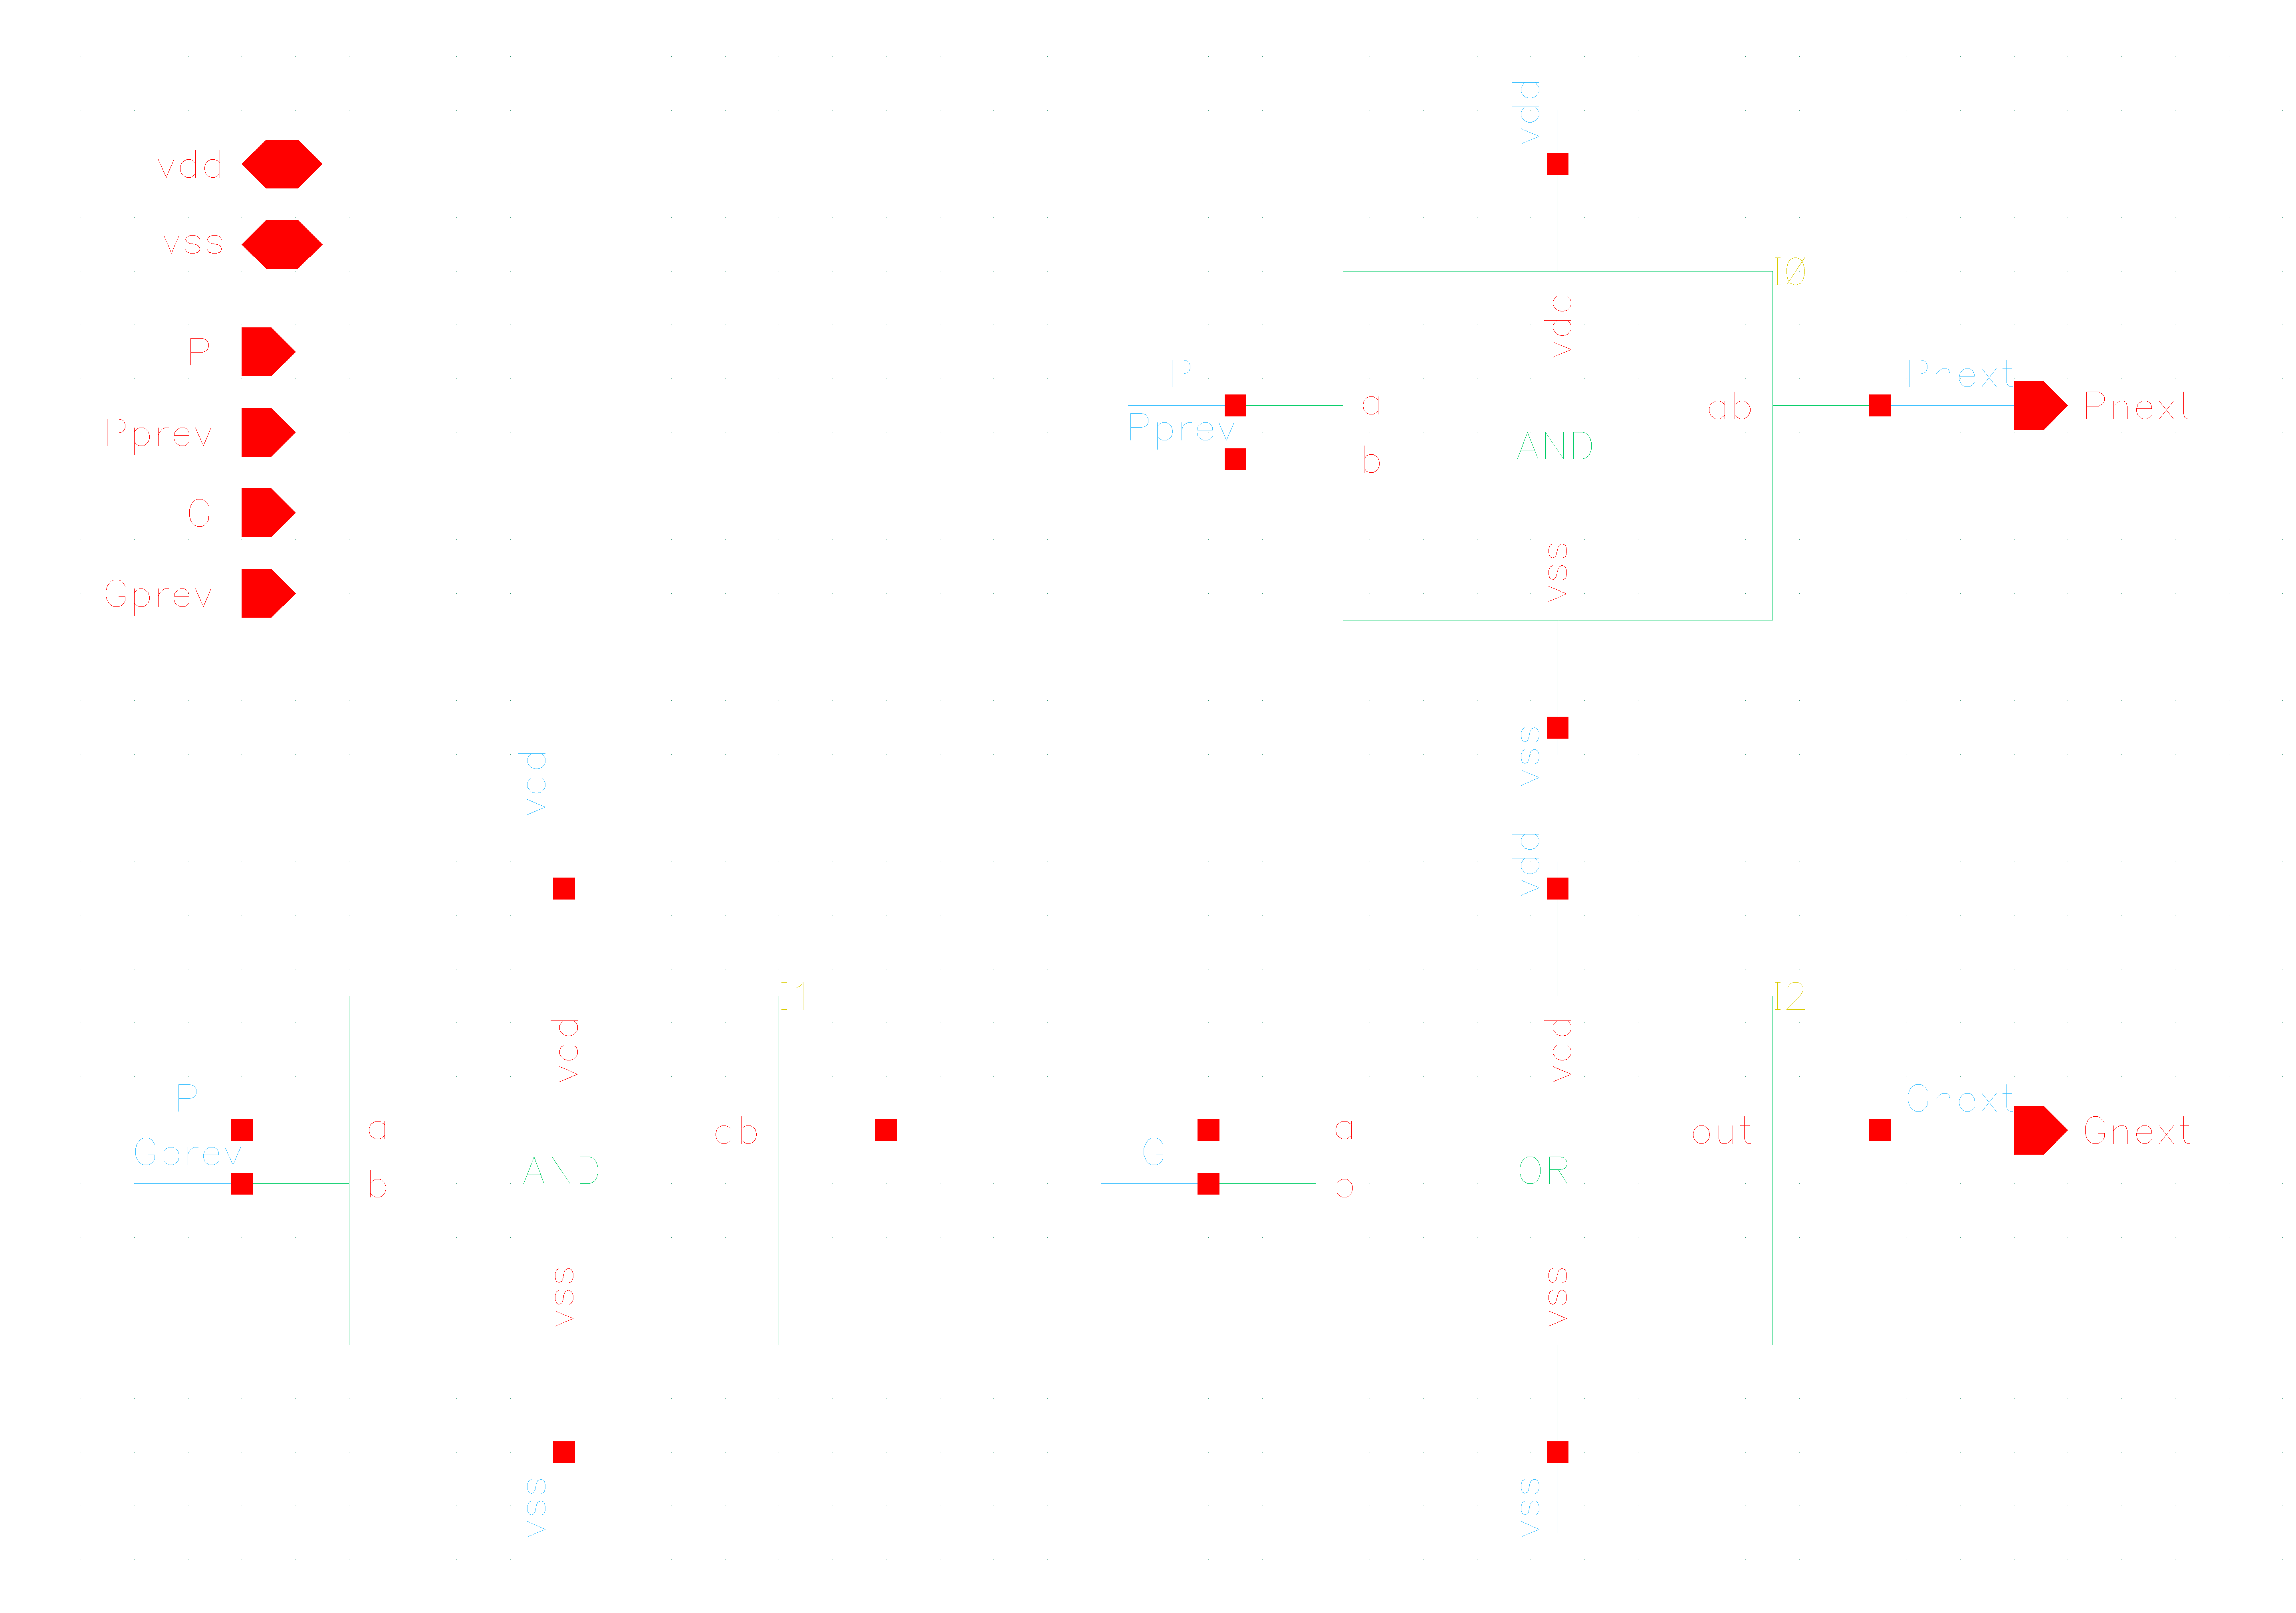
\includegraphics[width=1.3\textwidth]{../figures/yellow}}
  \caption{Schematic view of the yellow block.} \label{fig:yellow}
\end{figure}

\begin{figure}[H]
  \centering
  \captionsetup{justification=centering}
  \adjustbox{trim={.1\width} {0\height} {.1\width} {.4\height},clip}
  {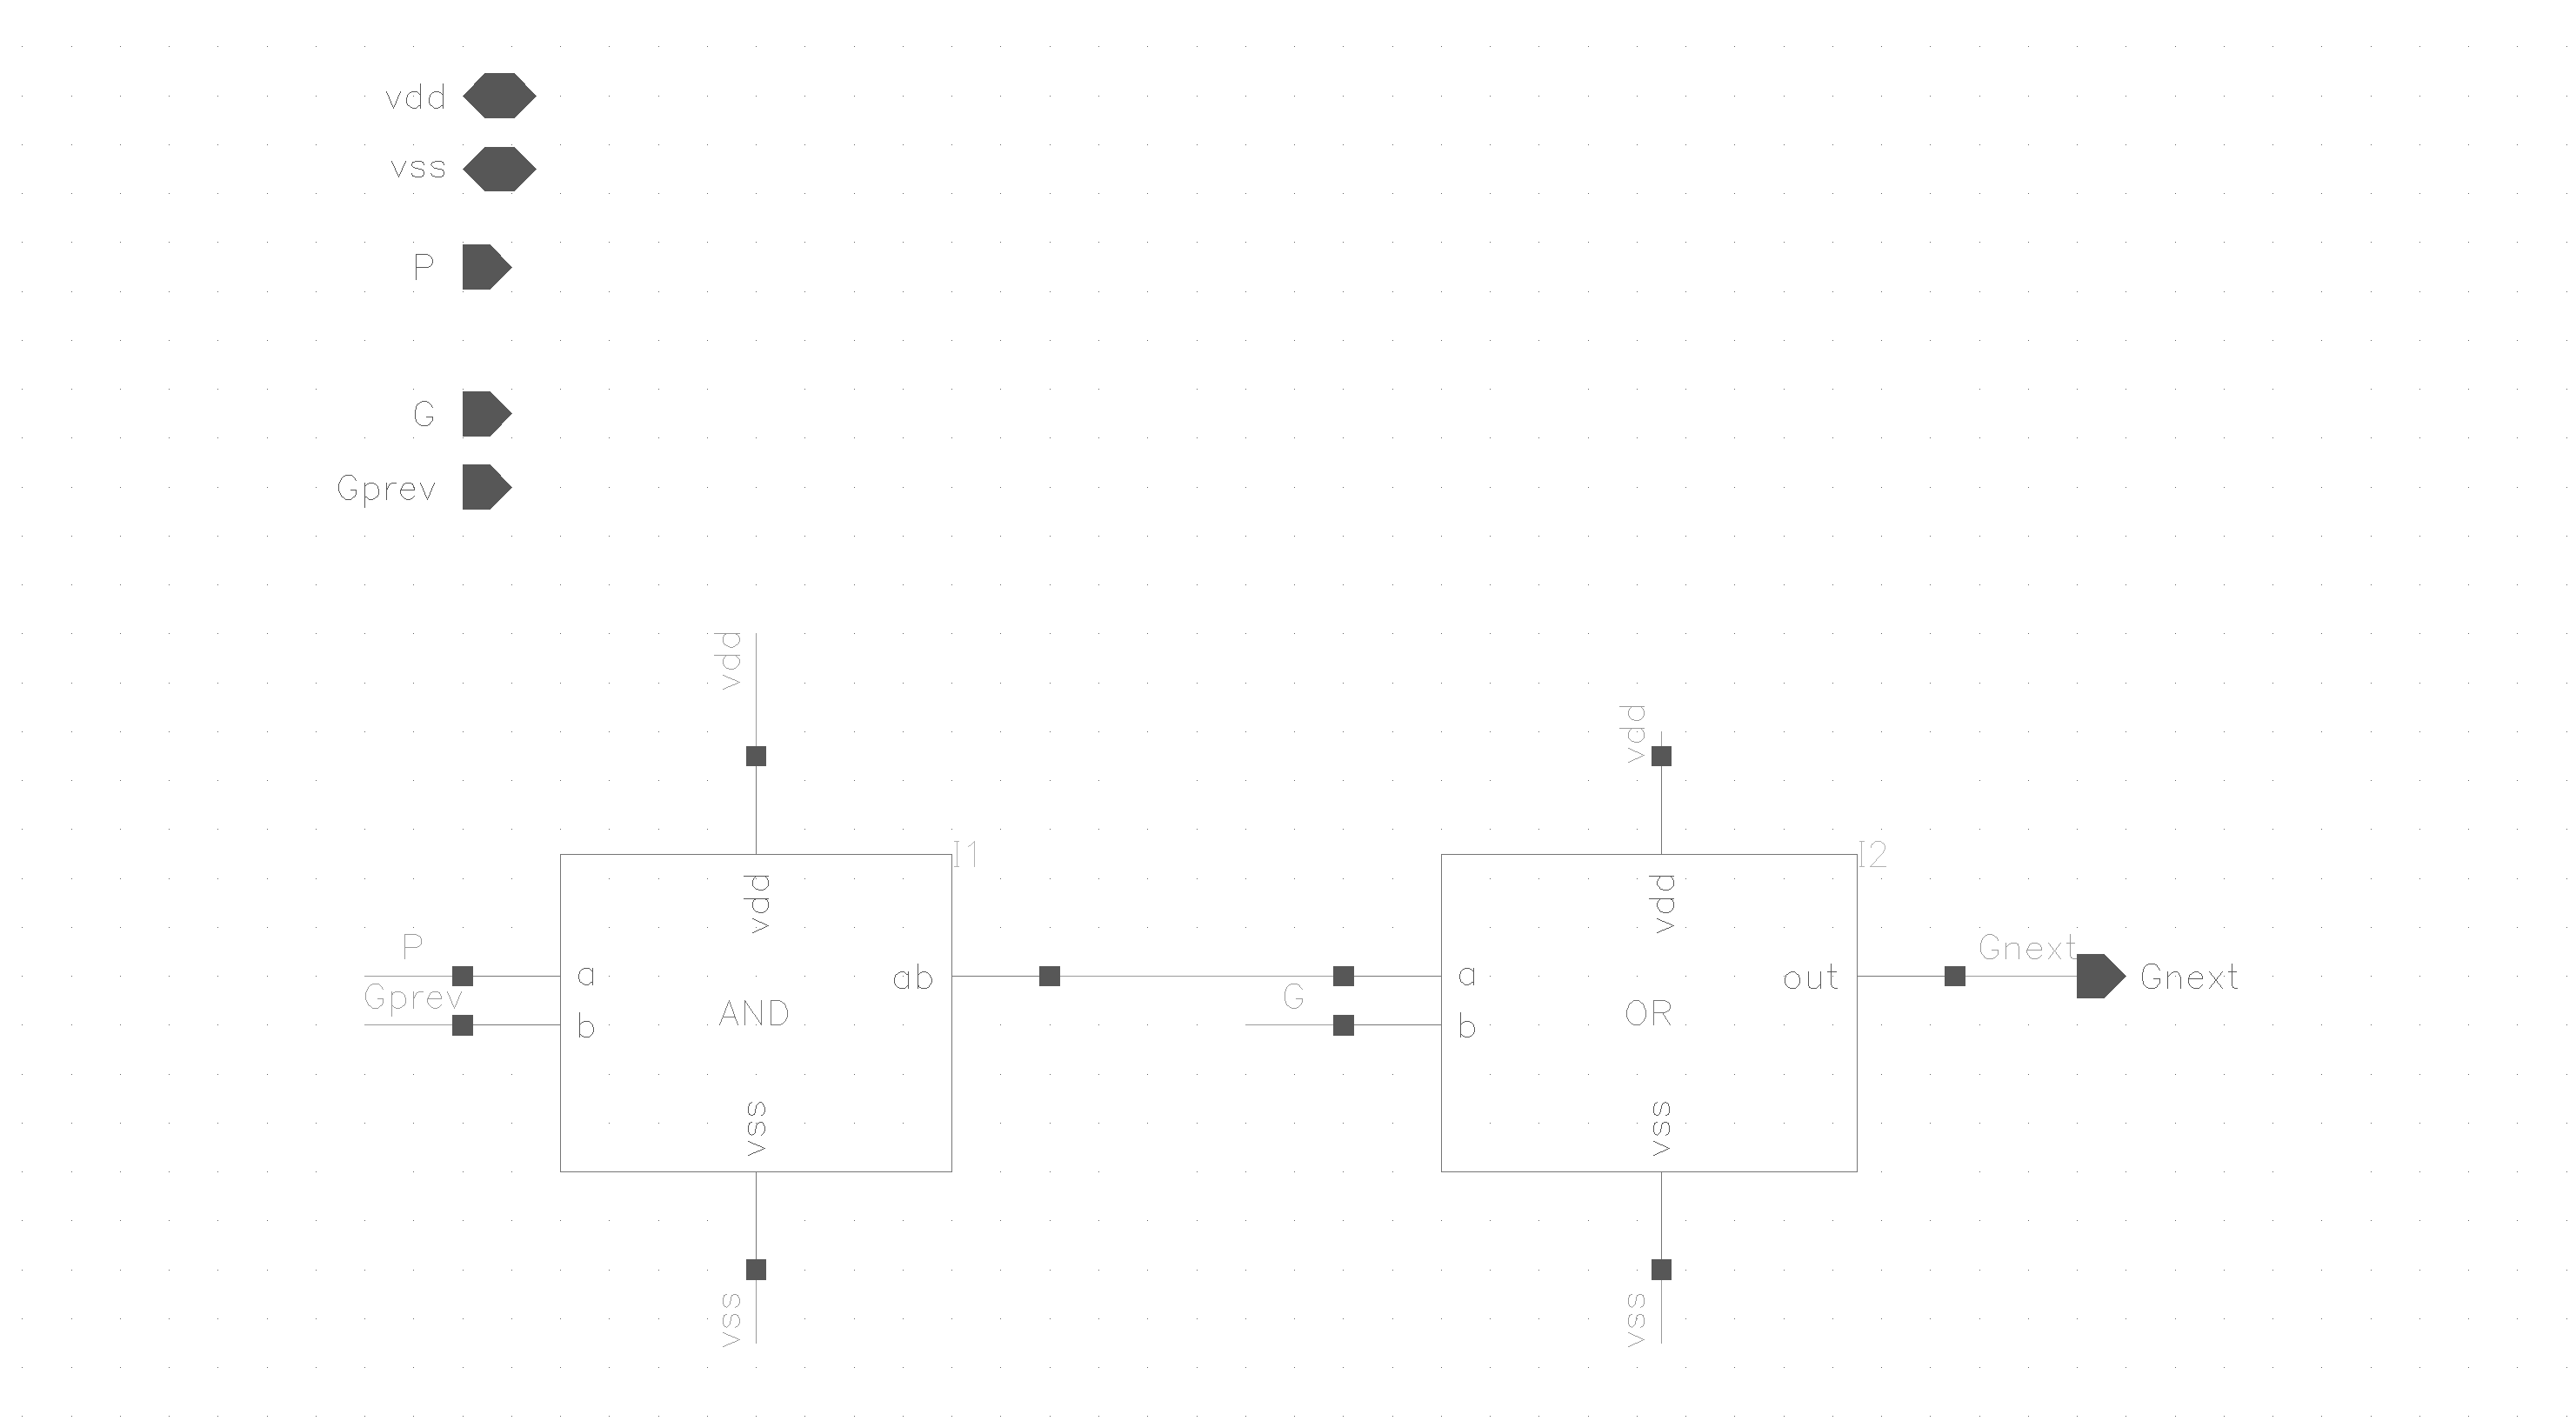
\includegraphics[width=1.2\textwidth]{../figures/yellow_carry}}
  \caption{Schematic view of the yellow carry block.} \label{fig:yellow_c}
\end{figure}

\begin{figure}[H]
  \centering
  \captionsetup{justification=centering}
  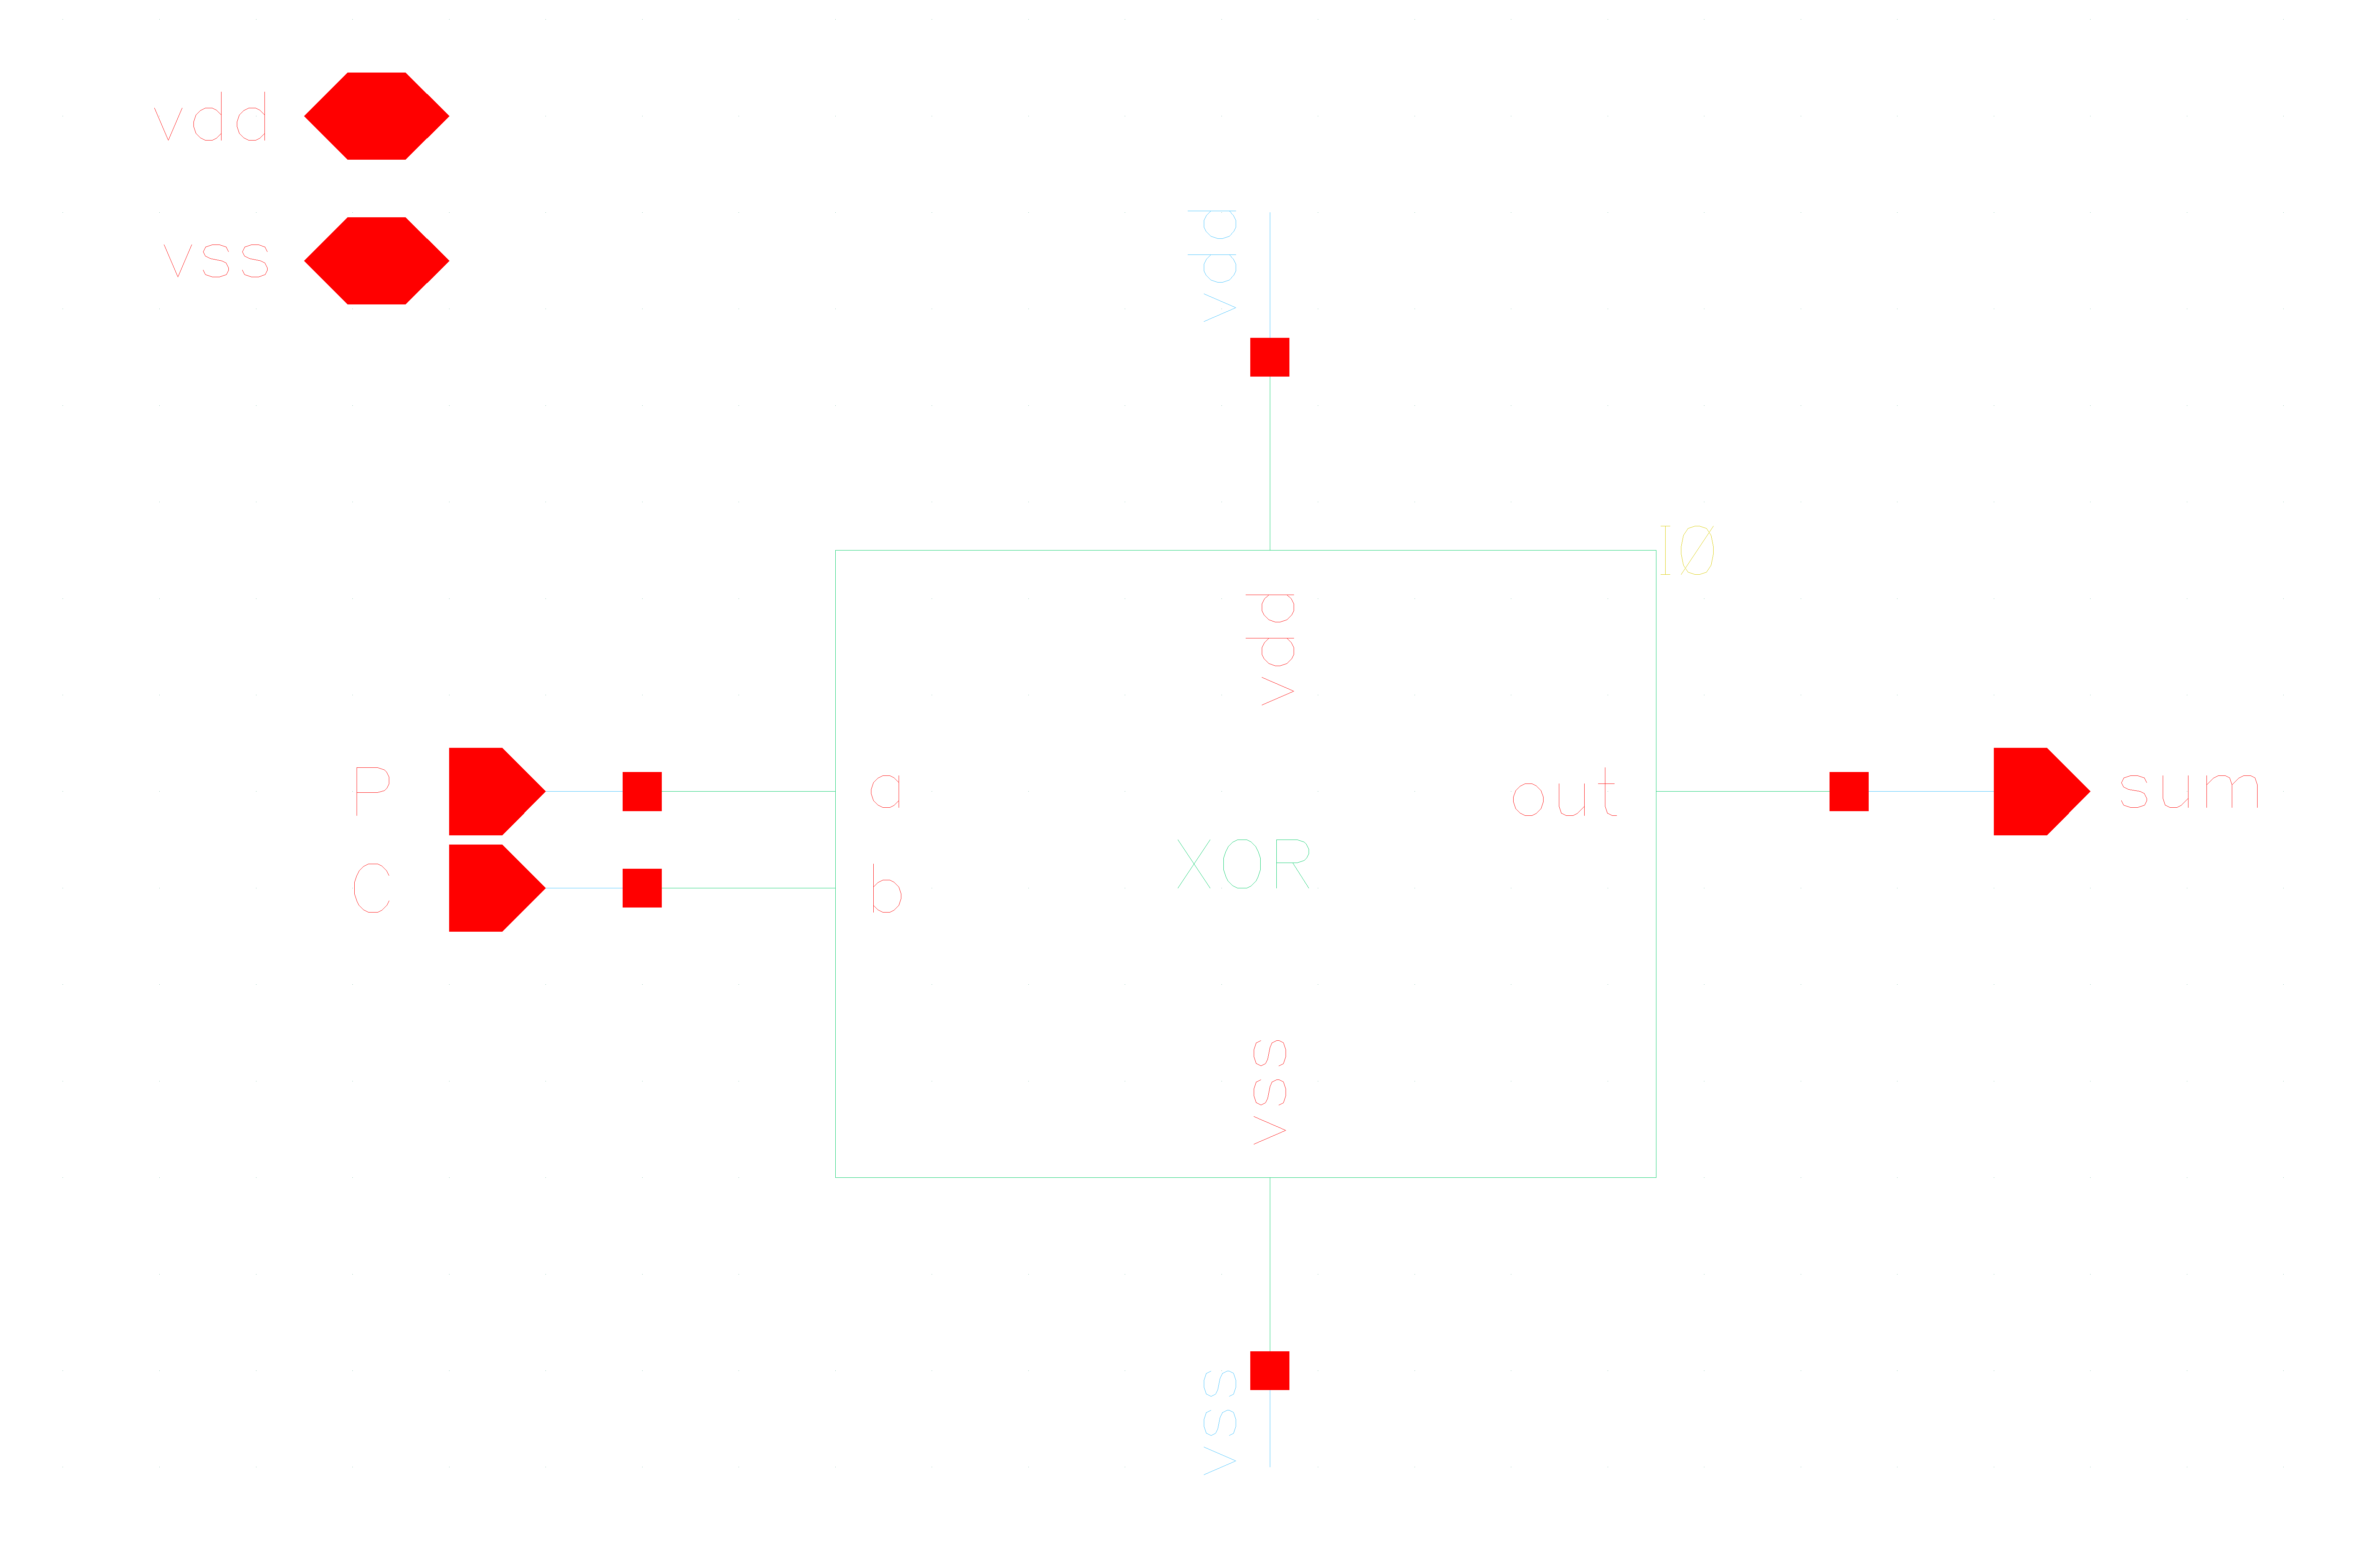
\includegraphics[clip,width=1.0\textwidth]{../figures/sum}
  \caption{Schematic view of the sum block.} \label{fig:sum}
\end{figure}

\subsection{Comparator}
The comparator consists of 17 2-input XNOR gates where one bit of each number is fed into each gate. The output from the XNOR gates are fed into a couple of AND gates which generates the final output. The comparator is 17 bits wide since it compares two 16 bit numbers plus their carry bits. The logic table of the XNOR gates is shown in table \ref{tab:xnor}.

\begin{table}[H]
  \caption{Logic table of XNOR block.}
  \centering
  \begin{tabular}{cc|c}
    \toprule
    $A_i$ & $B_i$ & $Y = \overline{(A_i \oplus B_i)}$ \\
    \midrule
    0 & 0 & 1 \\
    0 & 1 & 0 \\
    1 & 0 & 0 \\
    1 & 1 & 1 \\
    \bottomrule
    \label{tab:xnor}
  \end{tabular}
\end{table}



 \newpage
\subsection{SPI out}
This module is responsible for correctly outputtig data from the adder.


\subsubsection{Shift register}
The output consist of four sums, each containing 16 sum bits plus one carry output bit. This makes a total of 68 bits. To implement this we use a 68 bit shift register where each cell in the register contains one D flip-flop and one multiplexer. The multiplexer is used to switch between shifting and parallel load of the D flip-flop. In Fig. \ref{mux_dff} the schematic of some cells can be seen. 

\begin{figure}[H]
\centering
\captionsetup{justification=centering}
\includegraphics[scale=0.4]{../figures/spi_out_reg.png}
\caption{Shift register cell}
\label{mux_dff}
\end{figure}

\raggedright The spi enable signal is directly connected to the control signal of the multiplexer so that when spi enable is low, the input value to the D flip-flop is taken from the previous cell. 
 


\newpage

\subsubsection{Control logic}
The control logic is needed to load the long shift register with the correct data. \\
As the adder is built in such a way that it executes all the four additions as fast as it can after the spi enable signal goes high, the output from one addition will only be available for one system clock cycle. This means that we need to quickly grab the data and put it in the correct place.\\ 
Our implementation uses a pulse generator, a 2-bit counter, a decoder to select what 17-bit part of the shift register to load, and some multiplexers to select if to clock the register on the spi clock or on the enable signals from the decoder. The pulse generator is triggered by the spi enable signal and creates a pulse that is four system clock cycles long. This to only allow the counter to increment four times, and also to clip the pulse from the last decoder output. As can be seen in Fig. \ref{spi_out1} the last output of the decoder is also feeded back to the enable of the counter through an inverter. This prevents a possible glitch that is generated when the counter starts over. The glitch would reload the section of the shift register containing the first sum. \\

\begin{figure}[H]
\centering
\captionsetup{justification=centering}
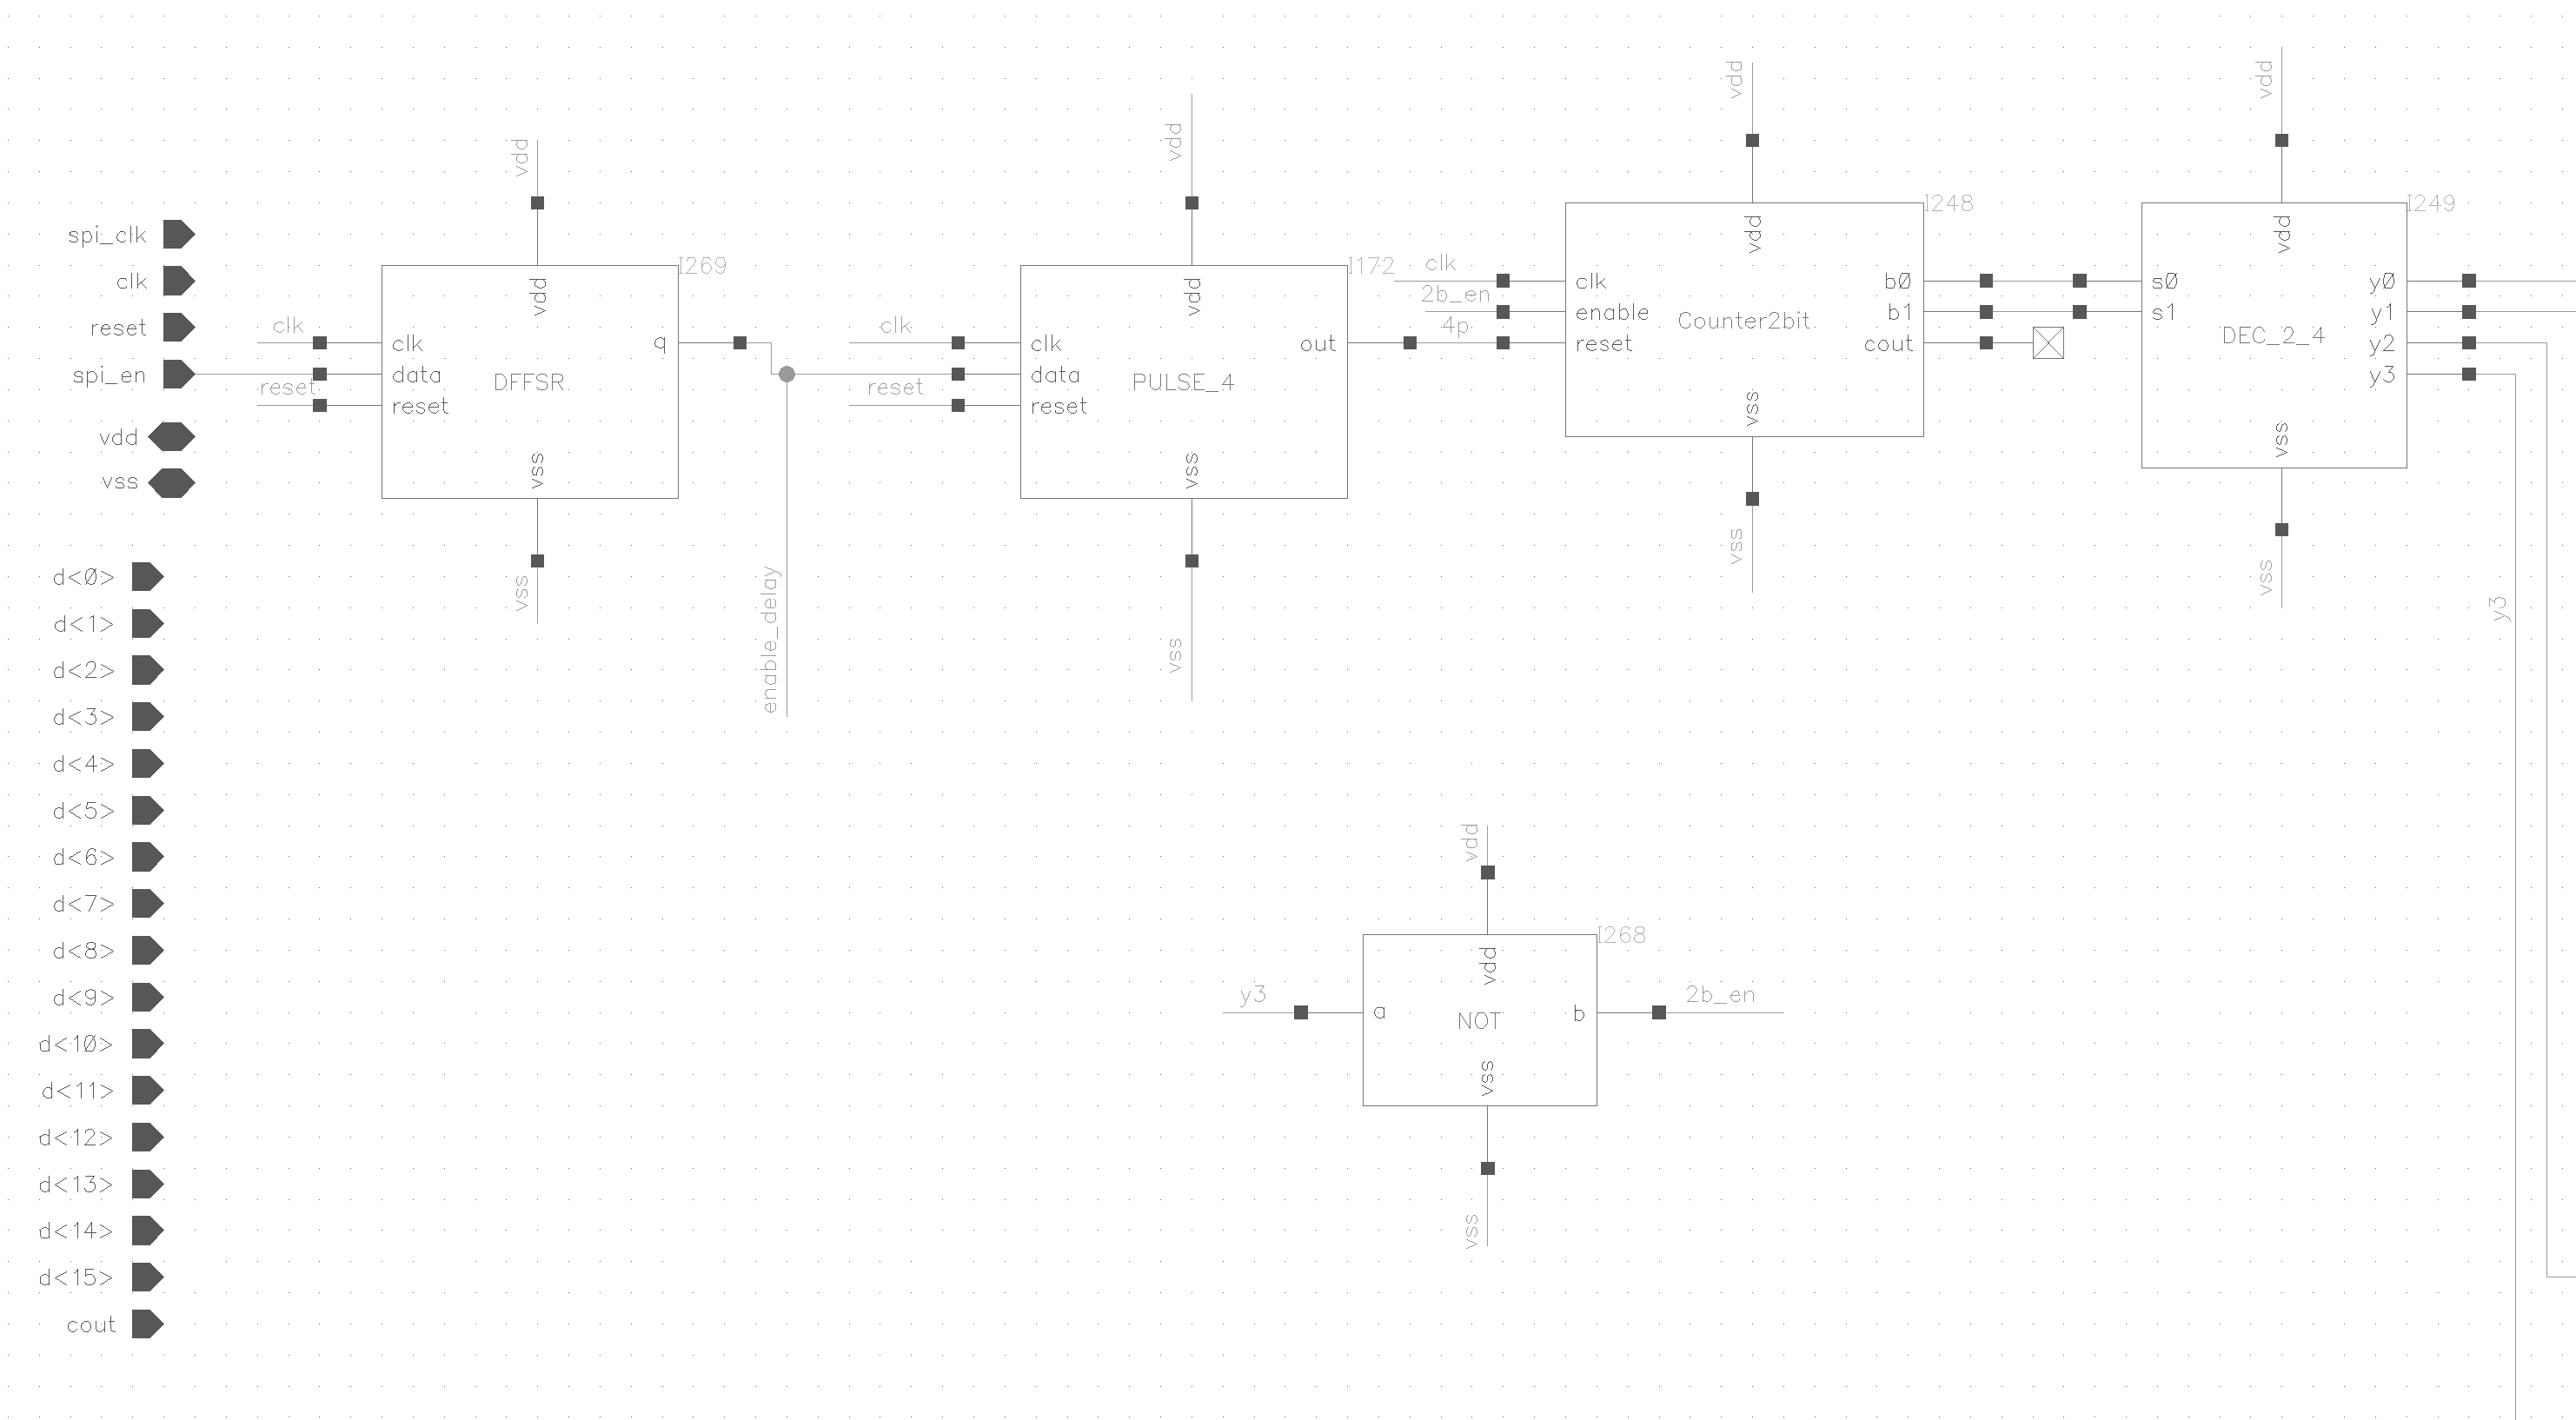
\includegraphics[scale=0.18]{../figures/spi_out1.png}
\caption{Control logic for spi output, first half}
\label{spi_out1}
\end{figure}

\newpage
\raggedright As can be seen to the right in Fig. \ref{spi_out2}, there are four enable signals: E1, E2, E3, E4. Each one of those signal enables a specific part of the shift register. If spi enable is low, all of the signals would be equal to the spi clock so that data can be shifted out. Otherwise, if the spi enable signal is high and, for example, E1 is high, the 17-bit part of the shift register corresponding to the sum of addition 1 would be loaded with the output from the adder.
\begin{figure}[H]
\centering
\captionsetup{justification=centering}
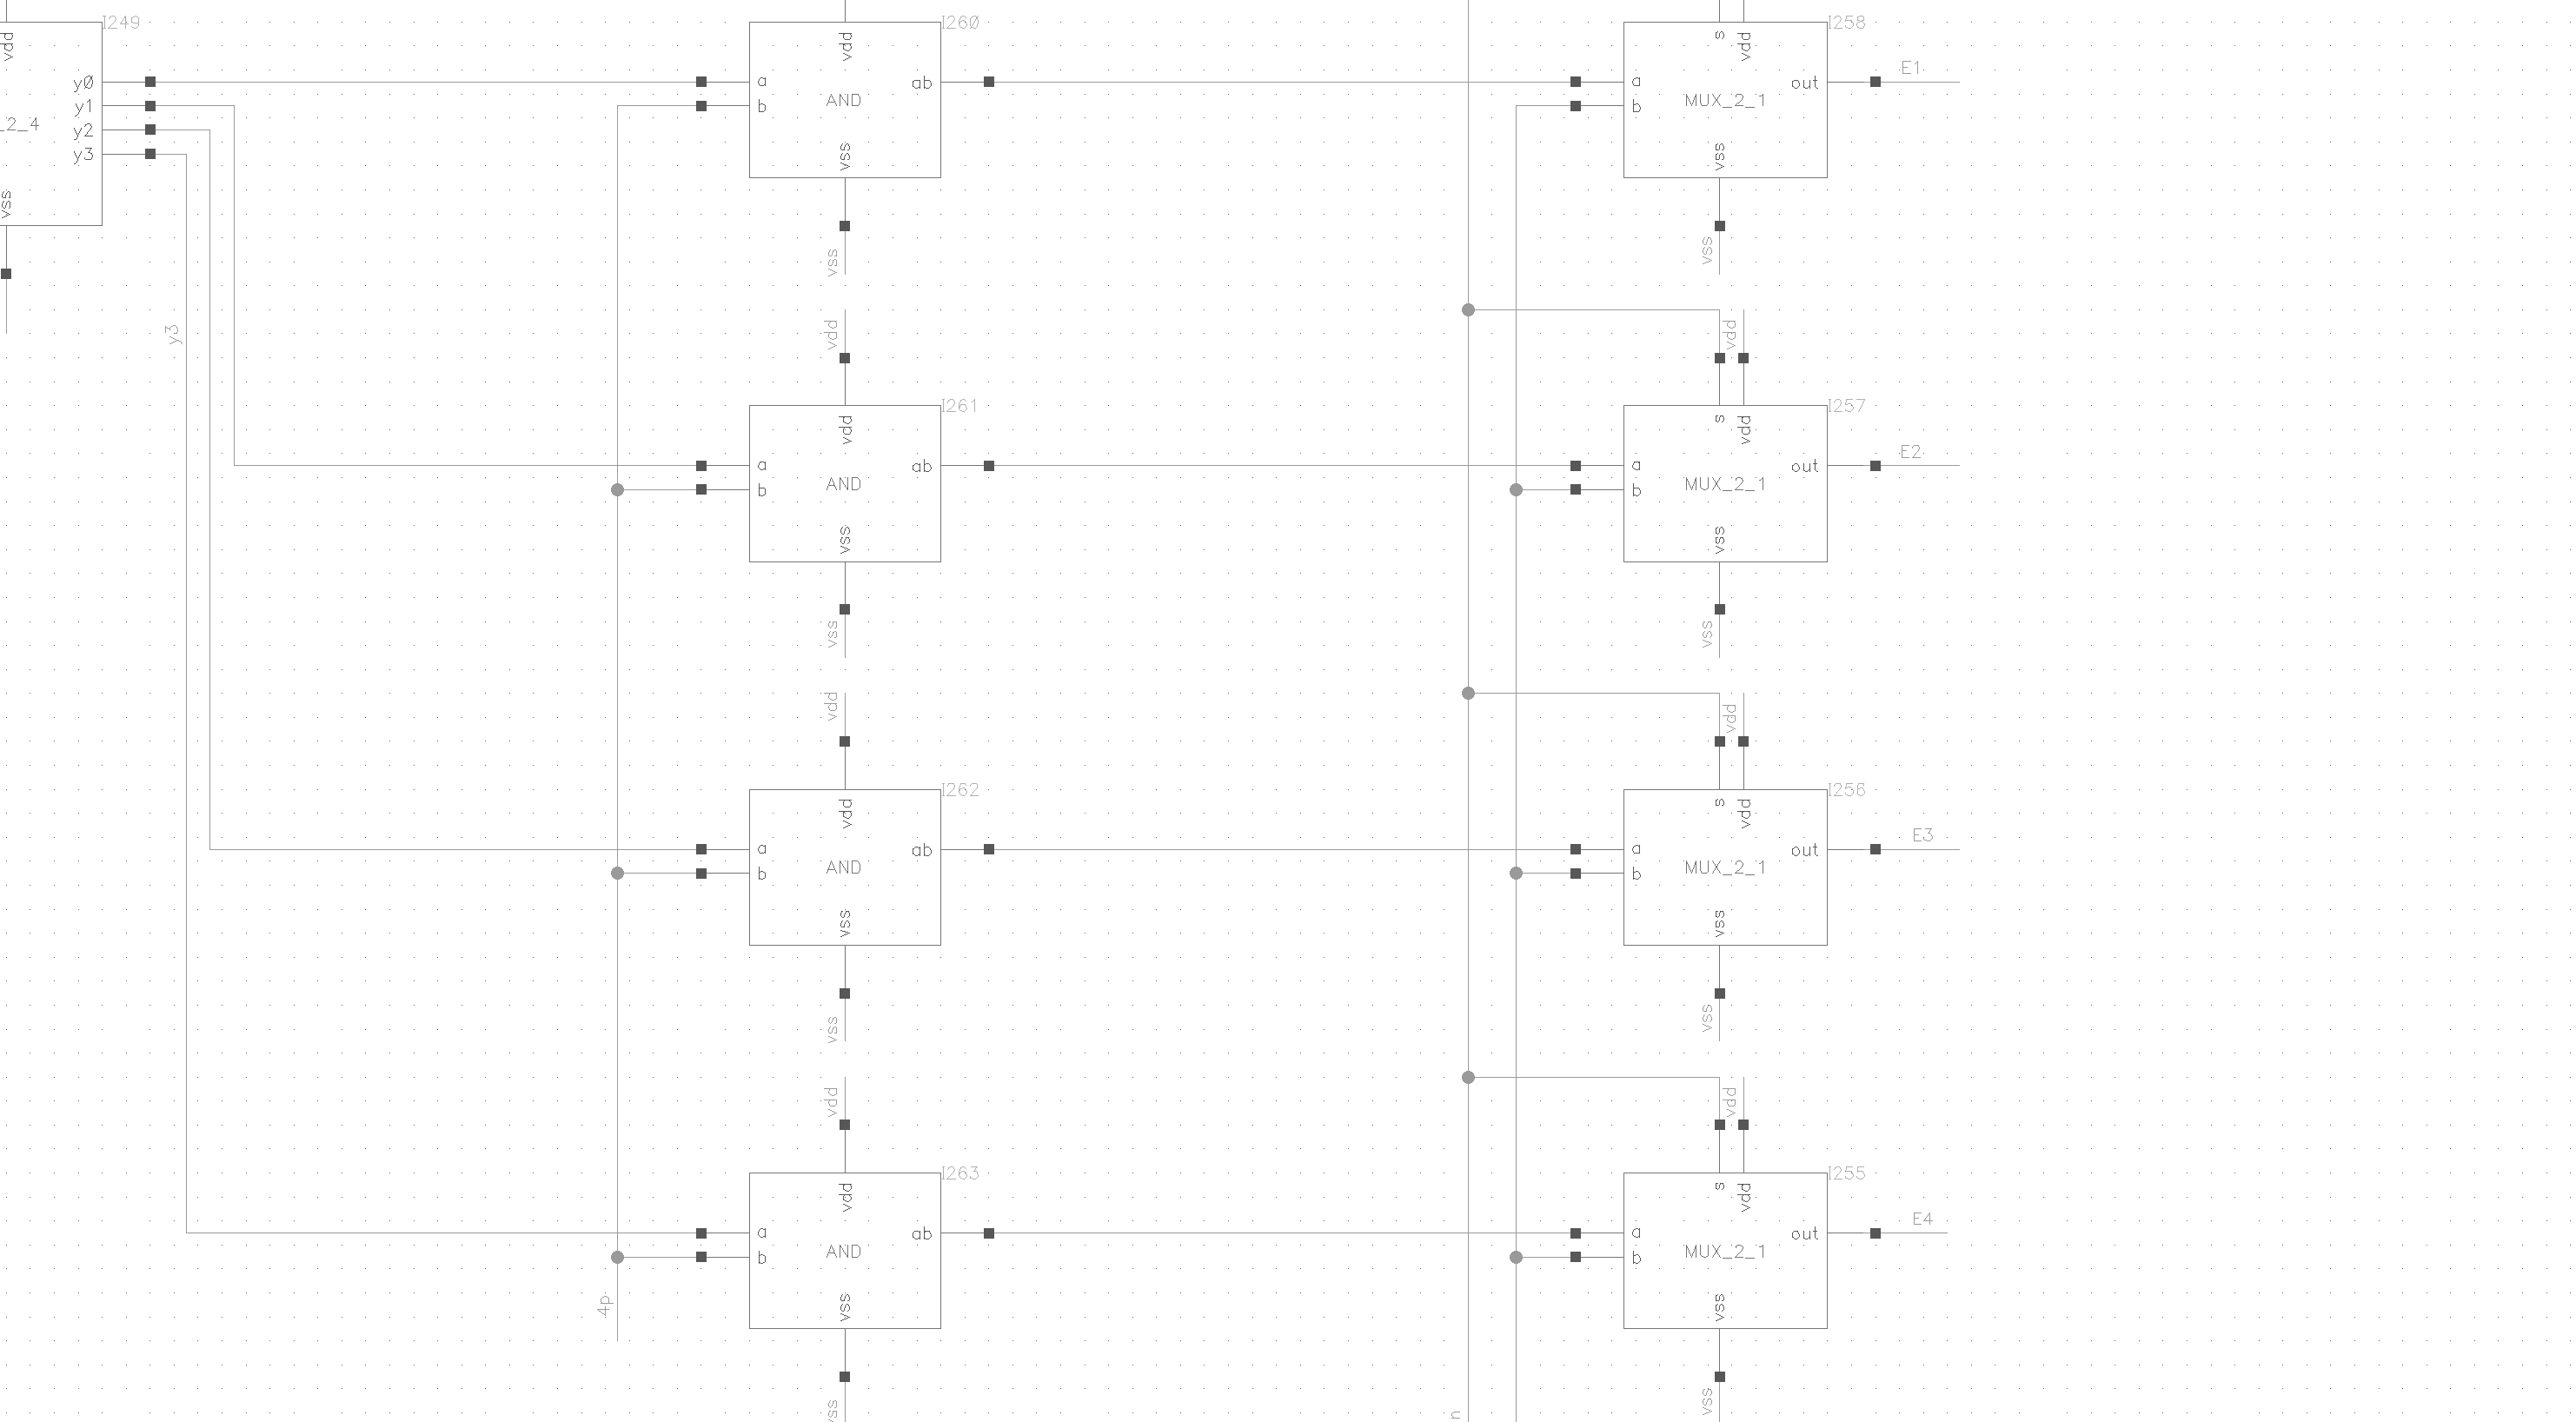
\includegraphics[scale=0.3]{../figures/spi_out2.png}
\caption{Control logic for spi output, second half}
\label{spi_out2}
\end{figure}

\subsection{Protocol}
This unit outputs the data with most significant bit first, in this case the carry output. To avoid using extra hardware, the group decided to go away from the standard spi protocol.  \\
Data is both written and read by the chip on the rising edge of the the spi clock. This means that the circuitry communicating with the chip has to read and write on the falling edge of the clock. Additionally, the first bit of the output will be available on the second falling edge after spi enable goes low.





\section{Simulation Results} \label{sec:simulation_results}
%This section describes the high level simulation results. As simulations with too many signals were consuming too much memory (and crashed) the group decided to only look at signals that showed if the chip worked or not.\\


%\subsection{Adder}
%In Fig. \ref{adder_sim} simulation of the propagation delay through the adder %can be seen. Due to routing problems it was shown that bit 8 of the sum were %the slowest and as can be seen, it takes approximately 2.7ns from system clock %edge until the result is ready. \\

%\subsection{SPI output}
%In Fig. \ref{spi_out_sim} the four enable signals, the spi clock and the spi enale signal from the spi output module is shown. As can be seen, the four enable signals each goes high once during the high period of the spi enable.\\
%When the spi enable signal goes low the most significant bit of the sum is available on the first falling edge of the spi clock. If you look closely, you can see that the first sum outputted are the same as the first correction sum that can be seen in table \ref{tab:test_data}. (all sums match except for the third correction sum which contains an error)\\

%\subsection{BIST}
%In Fig. \ref{bist_sim} a simulation of the BISTout signal can be seen. As mentioned earlier the correction sum contains an error which makes the BISTout signal go low for one cycle. \\
%It can also be seen that the BISTout first go high after two system clock cycles as effect from pipelining.\\

After running the simulation for different corners we retrieved the following data regarding system performance. The test data used can be seen in Tab. \ref{tab:test_data}.

\begin{table}[H]
	\caption{Corner results.}
	\centering
	\begin{tabular}{| l | c | c | c | c |}
		\hline
		Corner & Nominal & Worst speed & Worst power & Unit\\
		\hline
		Simulated temperature & $27$ & $100$ & $0$ & Celcius\\
		\hline 
		Tested frequency & $200$ & $166$ & $333$ & MHz  \\
		\hline
		Power consumption chip & $18.89$ & $16.54$ & $31.3$ & mW \\
		\hline 
		Power consumption adder & $0.93$ & $0.807$ & $1.436$ & mW \\
		\hline 
		Propagation delay sum15 & $2.209$ & $4.234$ & $1.264$ & ns \\
		\hline 
		Propagation delay cout & $2.195$ & $3.744$ & $1.332$ & ns \\
		\hline
		Possible adder frequency & $455$ & $236$ & $750$ & MHz \\
		\hline
	\end{tabular}
	\label{corner_result}
\end{table}

The propagation delay was measured between Cin and Cout and between Cin and Sum15. The possible adder frequencies in Tab. \ref{corner_result} are based on longest of these two. One thing to note is that the complete system did not function correctly during worst speed. The adder itself works fine and the correct data is outputted through SPI-out, but the built-in self test is failing.

Simulation results, for the nominal corner with a frequency of 200 MHz, of the propagation delay, the SPI-out data and of BISTout can be seen in Appendix \ref{app:simulations}.


\section{Pad Assignment and Early Test Plan}
The following signals will be connected to external pins on the chip, where the first seven are inputs and the last five are outputs:
\begin{itemize}
	\item Vdd1 - Will provide most of the system with power and will be a steady 3.3 V.
	\item Vdd2 - Will provide the adder with power and it might vary from 3.3 V downto below threshold-voltage
	\item GND - Ground
	\item Clk - This is the clock for the adder, some registers and control logic. Should have a frequency of at least 200 MHz at 3.3 V. Will be lower as we decrease the supply voltage.
	\item SPI\_clk - This clock is used by the input and output unit and should be at least five times slower than the system clock. Should also be low if SPI\_en is inactive.
	\item SPI\_en - Active low. Should go high on the first negative flank of SPI\_clk after the last value is read.
	\item SPI\_in - Updates it's value as soon as SPI\_en goes low, and should have it's value ready on the first positive flank of SPI\_clk, as this is when we read the value. The value of SPI\_in should then be updated on every negative flank of SPI\_clk.
	\item SPI\_out - The data is available for read on the first falling edge of SPI\_clk after SPI\_en has gone active.
	\item BIST\_out - If the in-data is correct, this should be constant high after the first addition is done. 
	\item Cin - Used to measure propagation delay.
	\item Cout - Used to measure propagation delay.
	\item Sum15 - Used to measure propagation delay.
\end{itemize}
 


\section{Risks and Delays}


\newpage

\begin{appendix}



\section{Block diagram of the Kogge-Stone Adder} \label{app:ks_block}

\begin{figure}[H]
  \centering
  \captionsetup{justification=centering}
  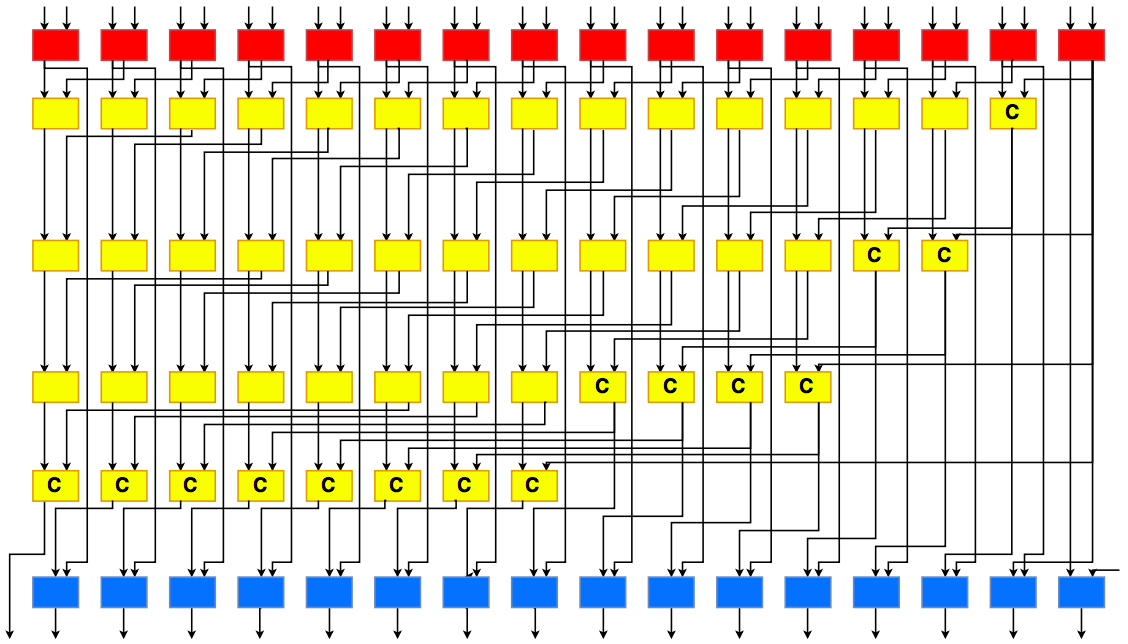
\includegraphics[scale=0.5, angle=90]{../figures/ks_block}
\end{figure}


\newpage

\section{Truth Tables for the Kogge-Stone Adder} \label{app:ks_truth}

\begin{table}[H]
  \caption{Logic table of red block.}
  \centering
  \begin{tabular}{cc|cc}
    \toprule
    $A_i$ & $B_i$ & $P=A_i \oplus B_i$ & $G=A_i \wedge B_i$ \\
    \midrule
    0 & 0 & 0 & 0 \\
    0 & 1 & 1 & 0 \\
    1 & 0 & 1 & 0 \\
    1 & 1 & 0 & 1 \\
    \bottomrule
    \label{tab:red}
  \end{tabular}
\end{table}

\begin{table}[H]
  \caption{Logic table of yellow block.}
  \centering
  \begin{tabular}{cccc|cc}
    \toprule
    $G_i$ & $G_{i,prev}$ & $P_i$ & $P_{i,prev}$ & $P=P_i \wedge P_{i,prev}$ & $G=(P_i \wedge G_{i,prev}) \vee G_i$ \\
    \midrule
    0 & 0 & 0 & 0 & 0 & 0 \\
    0 & 0 & 0 & 1 & 0 & 0 \\
    0 & 0 & 1 & 0 & 0 & 0 \\
    0 & 0 & 1 & 1 & 1 & 0 \\
    0 & 1 & 0 & 0 & 0 & 0 \\
    0 & 1 & 0 & 1 & 0 & 0 \\
    0 & 1 & 1 & 0 & 0 & 1 \\
    0 & 1 & 1 & 1 & 1 & 1 \\
    1 & 0 & 0 & 0 & 0 & 1 \\
    1 & 0 & 0 & 1 & 0 & 1 \\
    1 & 0 & 1 & 0 & 0 & 1 \\
    1 & 0 & 1 & 1 & 1 & 1 \\
    1 & 1 & 0 & 0 & 0 & 1 \\
    1 & 1 & 0 & 1 & 0 & 1 \\
    1 & 1 & 1 & 0 & 0 & 1 \\
    1 & 1 & 1 & 1 & 1 & 1 \\
    \bottomrule
    \label{tab:yellow}
  \end{tabular}
\end{table}

\begin{table}[H]
  \caption{Logic table of yellow with carry block.}
  \centering
  \begin{tabular}{ccc|c}
    \toprule
    $P_i$ & $G_i$ & $G_{i,prev}$ & $G=(P_i \wedge G_{i,prev}) \vee G_i$  \\
    \midrule
    0 & 0 & 0 & 0 \\
    0 & 0 & 1 & 0 \\
    0 & 1 & 0 & 1 \\
    0 & 1 & 1 & 1 \\
    1 & 0 & 0 & 0 \\
    1 & 0 & 1 & 1 \\
    1 & 1 & 0 & 1 \\
    1 & 1 & 1 & 1 \\
    \bottomrule
    \label{tab:yellowcarry}
  \end{tabular}
\end{table}

\begin{table}[H]
  \caption{Logic table of sum block.}
  \centering
  \begin{tabular}{cc|c}
    \toprule
    $P_i$ & $C_{i-1}$ & $S_i=P_i \oplus C_{i-1}$ \\
    \midrule
    0 & 0 & 0 \\
    0 & 1 & 1 \\
    1 & 0 & 1 \\
    1 & 1 & 0 \\
    \bottomrule
    \label{tab:sum}
  \end{tabular}
\end{table}


\newpage

\section{Time Plan} \label{app:time_plan}

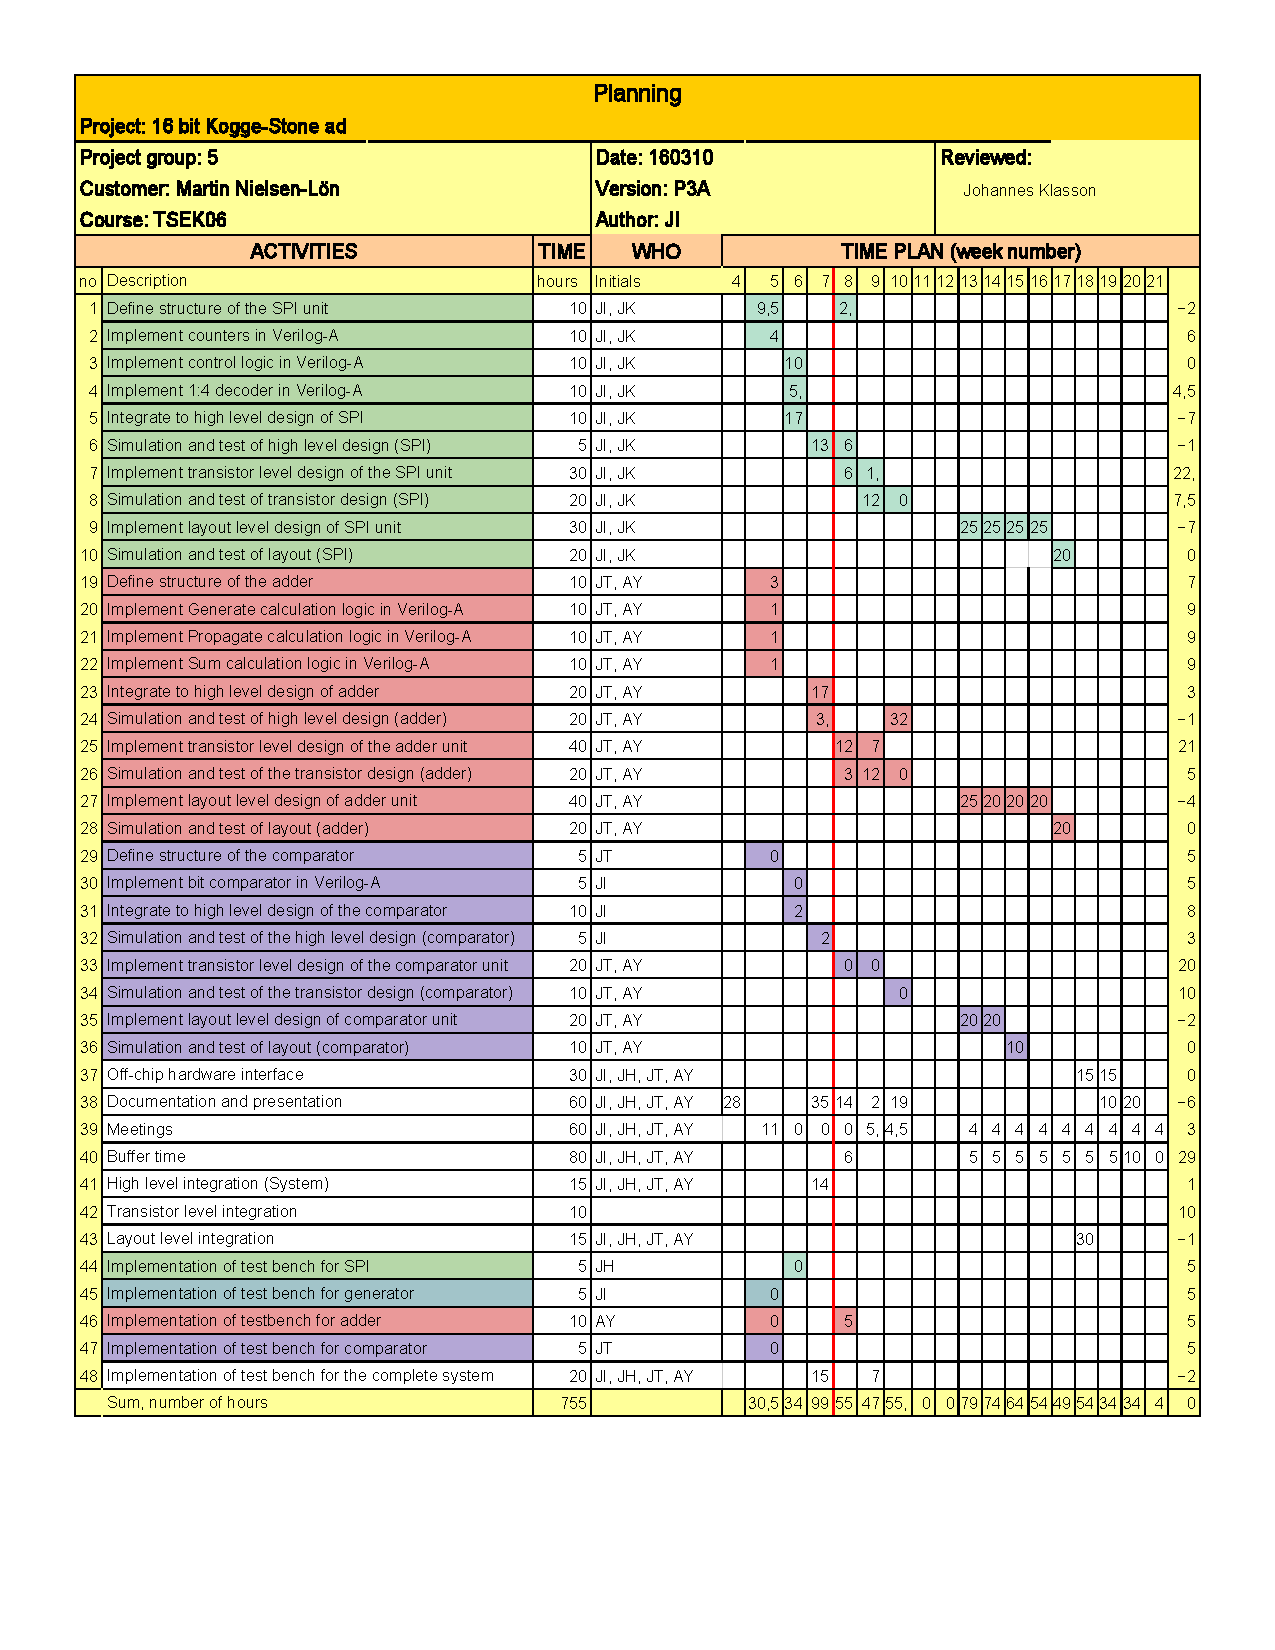
\includegraphics[scale=0.7]{../figures/TSEK06_G05_timeplan_P3A.pdf}

\newpage

%\section{Time Report} \label{app:time_report}
\todo{JOHAN}

%\newpage

\end{appendix}
\end{document}
